%%
%% Author: dariochinelli
%% from 2020-09-29 to 2021-03-30
%%

% Preamble
\documentclass[11pt]{article}

% Packages
\usepackage[top=1in, bottom=1in, left=1in, right=1in]{geometry}
\usepackage{amsmath}
\usepackage{enumitem}
\usepackage{amssymb}
\usepackage{tikz}
\usepackage{siunitx}
\usepackage{imakeidx}
\usepackage{graphicx}
\graphicspath{ {img/} }
\usepackage{color}   %May be necessary if you want to color links
\usepackage{hyperref}
\hypersetup{
    colorlinks=true, %set true if you want colored links
    linktoc=all,     %set to all if you want both sections and subsections linked
    linkcolor=blue,  %choose some color if you want links to stand out
}

% Document
\begin{document}

\title{\textbf{Appunti di Struttura della Materia 1}} 

\author{Manoscritto e diretto da \textbf{Alessandro Greco} nel 2018. \\
Scritto in \LaTeX\ aggiornato e corretto da \textbf{Dario Chinelli} nel 2021.}

\date{30 marzo 2021}

\maketitle

    \newpage

    \tableofcontents

    %%
%% Author: dariochinelli
%% 2021-03-10
%%
\section{Varie info utili}
Riassumo qui molte delle formule ricavate e le costanti utilizzate nei paragrafi successivi.
\subsection{Formule}
\begin{equation}
\begin{split}
\mbox{Legge di Wien} & \quad \lambda_{max} T = \SI{2.898e-3}{m*K} = \mbox{ } const \\
\mbox{Legge di Stefan-Boltzmann} & \quad R_T = \sigma T^4 \\
\mbox{Densità energia Corpo Nero Raylight-Jeans} & \quad \rho_T d\nu = \frac{ 8 \pi \nu^2}{c^3 } kT d\nu \\
\mbox{Densità energia Corpo Nero Planck} & \quad  \rho_T d\nu = \frac{ 8 \pi \nu^2}{c^3 }\frac{ h\nu}{e^{ \frac{ h\nu}{kT } } - 1 } d\nu  \\
\mbox{Densità energia $\propto$ Radianza} & \quad \frac{ c}{4 } \rho_T(\nu) = R_T(\nu) \\
\mbox{Energia effetto fotoelettrico} & \quad K_{max} = h\nu - W_0 = eV_0 \\
\mbox{Variazione lunghezza d'onda effetto Compton} & \quad \Delta \lambda = \frac{ h}{m_{e} c } (1 - \cos \theta) = \lambda_c (1 - \cos \theta) \\
\mbox{Diffrazione differenza cammino ottico} & \quad \Delta = 2 d \sin \theta = n \lambda \\
\mbox{Equazione equil mecc elettrone (Bohr)} & \quad 
\begin{cases}
	F_{coul} = \frac{ 1}{4 \pi \varepsilon_0 } \frac{ Z e^2}{r^2 } = m \frac{ v^2}{r } = F_{cent} \\
	L = m v r =  n \hbar
\end{cases} \\
\mbox{Energia livelli orbitali (Bohr)} & \quad E = -\frac{ 1}{8 } \frac{ m e^4}{\varepsilon_0^2 h^2 } \frac{ Z^2}{n^2 } \\
\mbox{Regola di Wilson-Sommerfeld} & \quad \oint P_q dq = n_q h \\
\mbox{Hamiltoniana/Energia oscillatore armonico} & \quad H = E = K + V = \frac{ P_x^2}{2m } + \frac{ k x^2}{2 } \\
\mbox{Calore specifico Dulong-Petit} & \quad C_V = 3R \quad T \gg 0 \\
\mbox{Calore specifico Einstein} & \quad C_V = \frac{ 3 N_A (h\nu)^2}{kT^2 } e^{ -\beta h \nu } \quad \mbox{quasi-ovunque} \\
\mbox{Calore specifico Debye} & \quad C_V = 
	\begin{cases}
		\frac{ 12}{5 } \pi^4 R \Bigl(  \frac{ T}{\Theta }  \Bigr)^3 \quad \mbox{contrib. reticolare} \\
		\frac{ \pi^2}{2 } N k \Bigl(  \frac{ T}{T_F}  \Bigr) \quad \mbox{contrib. elettronico} 
	\end{cases} \\
\end{split}
\end{equation}

\subsection{Costanti}
\begin{equation}
\begin{split}
\mbox{Massa elettrone} & \quad m_e = \SI{9.1e-31}{Kg} \\
\mbox{Carica elettrone} & \quad e = \SI{1.602e-19}{C} \\
\mbox{Costante dielettrica vuoto} & \quad \varepsilon_0 = \SI{8.854e-12}{F/m} \\
\mbox{Costante di Planck} & \quad h = \SI{6.626e-34}{J s} \\
\mbox{Costante di Planck ridotta} & \quad \hbar = \frac{ h}{2\pi } = \SI{1.0545e-34}{J s} \\
\mbox{Energia minima idrogeno} & \quad \frac{ 1}{8 }\frac{m e^4 }{\varepsilon_0^2 h^2 } \Bigl(  \frac{ Z^2}{n^2 }  \Bigr)= \SI{-13.6e0}{eV} \\
\mbox{Costante di Stefan-Boltzmann} & \quad \sigma = \SI{5.67e-8}{W / ( m^2 K^4)} \\
\mbox{Costante di Boltzmann} & \quad k_B = k = \SI{1.3806e-23}{J / K} \\
\mbox{Numero (costante) di Avogadro} & \quad N_A = \SI{6.02214076e23}{mol^{-1}} \\
\mbox{Conversione J - eV} & \quad \SI{1 }{eV} = \SI{1.6022e-19}{J} \\
\mbox{Lunghezza d'onda di Compton} & \quad \lambda_c = \frac{ h}{m_e c } = \SI{2.4263e-12}{m} \\
\end{split}
\end{equation}


%\iffalse
    %%
%% Author: dariochinelli
%% 2021-04-03
%%


\section{Il corpo nero}
Il corpo nero è un concetto utile per descrivere un oggetto le cui pareti si trovino a temperatura $T$ uniforme e costante, esso emette uno spettro di radiazione continuo che dipende solamente dalla temperatura e non dal materiale di cui è composto.
Le cariche elettriche costituenti le pareti si muovono in virtù dell'agitazione termica e così facendo irraggiano onde elettromagnetiche che vanno riempiendo la cavità: in questo modo si trasferisce energia dalle pareti al campo elettromagnetico al suo interno.
Tali onde elettromagnetiche a loro volta urtando contro le pareti trasferiscono energia dal campo elettromagnetico alle pareti.
Quando si raggiunge l'equilibrio termico tra le onde all'interno e le pareti dell'oggetto si ha che l'energia ricevuta è uguale a quella emessa.\\
\textbf{Definiamo} \\
\underline{\textit{Radianza Spettrale}}: $R_T(\nu)$ potenza su area, ovvero energia emessa per unità di tempo nell'intervallo di frequenze tra $\nu$ e $\nu+d\nu$ da un'area unitaria di superficie ad una certa temperatura $T$. \\
\underline{\textit{Radianza Totale} o \textit{Radianza}}: $R_T= \int_0^{\infty} R_T(\nu)d\nu$ integrale su tutte le frequenze della radianza spettrale, descrive l'energia totale per unità di tempo di un'area unitaria di superficie ad una certa temperatura $T$.
\begin{figure}[h]
\centering
\includegraphics[scale=0.6]{/Spectral_radiancy}
\caption{Radianza spettrale di corpo nero a tre diverse temperature. Notare come il picco si sposti all'aumentare della temperatura.}
\end{figure}
Per descrivere la radiazione di corpo nero Rayleigh e Jeans utilizzarono (anche) le seguenti leggi empiriche:
la \textbf{legge di Stefan-Boltzmann}:
\begin{equation}
R_T = \sigma T^4
\end{equation}
che descrive la radianza totale in funzione della temperatura ed in cui compare la 
\begin{equation}
\mbox{\underline{costante di Stefan-Boltzmann}} \quad \sigma = 5.67 \cdot 10^{-8} \frac{W}{m^2 \cdot K^4}
\end{equation}
La \textbf{legge di spostamento di Wien} afferma che la frequenza di picco è proporzionale alla temperatura
\begin{equation}
\begin{split}
& \nu_{max} \propto T \\
& \mbox{ed usando la seguente relazione} \quad \lambda\nu = c \\
& \lambda_{max}T = \SI{2.898e-3}{mK}
\end{split}
\end{equation}
L'oggetto reale più simile al concetto teorico di corpo nero è la \underline{cavità di corpo nero}, cioè un oggetto cavo con pareti metalliche avente un piccolo buco sulla superficie: la radiazione che esce dal foro è interpretabile come corpo nero, vedi figura.
\begin{figure}[h]
\centering
\includegraphics[scale=0.6]{/cavita_corponero}
\end{figure}
Introduciamo la \underline{\textbf{radiazione di cavità}} $\rho_T(\nu)$, che è la densità di energia contenuta in una unità di volume della cavità ad una certa temperatura $T$,
essa è ovviamente proporzionale alla Radianza totale, la cui derivazione è basata su ragionamenti puramente geometrici, in particolare la relazione è data da:
\begin{equation}
\frac{c}{4}\rho_T(\nu)=R_T(\nu)
\end{equation}


\subsection{Teoria classica di corpo nero di Rayleigh e Jeans}
A inizio '900 spiegare la forma dello spettro di corpo nero era uno dei problemi più dibattuti.
A dare un grande contributo furono Rayleigh e Jeans, che elaborarono la teoria classica di corpo nero, basandosi sulla fisica classica, per modellizzare la forma dello spettro di corpo nero.
Quindi si impegnarono nel trovare un modello teorico che potesse spiegare i risultati sperimentali. \\
Il ragionamento si divide in tre passaggi:
\begin{enumerate}[label=\Roman{*}.]
\item Le onde elettromagnetiche all'interno della cavità sono onde stazionarie?
\item Come contare il numero di onde stazionarie?
\item È possibile associare un'energia alle onde elettromagnetiche?
\end{enumerate}
\begin{figure}[h]
\centering
\includegraphics[scale=0.7]{/cubo_CorpoNero}
\caption{cubo Corpo Nero}
\end{figure}
Si consideri una cavità cubica e metallica riscaldata a temperatura $T$.
Essi ragionarono con le frequenze delle onde elettromagnetiche contenute nella cavità.
Vediamo in dettaglio i passaggi seguiti da Rayleigh e Jeans.
\begin{enumerate}[label=\Roman{*}.]
\item Prima di tutto occorre dimostrare che tali onde siano stazionarie.
Ogni onda può essere scomposta lungo le tre componenti spaziali e studiata indipendentemente. 
Consideriamo il lato del cubo $x \in (0, a)$.
La radiazione elettromagnetica è trasversale, cioè il campo elettrico $\vec{E}$ è perpendicolare alla direzione di propagazione dell'onda, dunque il campo è parallelo alla parete, ma ciò porta all'annullarsi di $\vec{E}$ sulla parete, perciò sui lati del cubo deve esserci ampiezza nulla, e quindi $0$ e $a$ sono due nodi.
Le onde sono dunque stazionarie.
\begin{figure}[h]
\centering
\includegraphics[scale=0.6]{/modiVibrazione}
\caption{modi vibrazione}
\end{figure}
\item Occorre contare il numero di onde, cominciamo dal caso 1-D lungo $x$
\begin{equation}
\begin{split}
& E(x, t) = E_0 \sin \Bigl(  \frac{2 \pi x}{\lambda}  \Bigr) \sin (2\pi \nu t) \\
& \frac{2x}{\lambda} = 0,1,2,3 ... = n \in \mathbb{N}
\end{split}
\end{equation}
Quindi $n=0$ corrisponde all'estremità, fissa, in $x=0$ e tutte le possibili onde stazionarie si trovano imponendo $x=a$:
\begin{equation}
\begin{split}
& \frac{ 2a}{\lambda } = n \quad\quad n = 1,2,3, ... \\
& \mbox{utilizzando la relazione} \quad \nu = \frac{c}{\lambda} \\
& \nu = \frac{ c n }{2a } \quad n = 1,2,3, ...
\end{split}
\end{equation}
Che sono quindi i valori permessi di frequenza per onde stazionarie.
\begin{figure}[h]
\centering
\includegraphics[scale=0.7]{/Blackbody_nodi}
\end{figure}
\begin{equation}
\begin{split}
& d = (\frac{ 2a}{c }) (\nu + d\nu) \quad - \quad d = (\frac{ 2a}{c }) \nu \\
& N(\nu)d\nu = 2 \Bigl(  \frac{2a}{c}  \Bigr) d\nu = \frac{4a}{c}d\nu 
\end{split}
\end{equation}
Nel caso unidimensionale questo è il numero di modi di vibrazione, dove il fattore 2 è dovuto al fatto che ci siano due possibili polarizzazioni $S$ e $P$. \\
\textbf{NB} Nel caso 1-D il numero di frequenze possibili non dipende da $\nu$.
Passiamo a 3 dimensioni, il valore di $n$ dipenderà ora da tre parametri $n_x, n_y, n_z \in \mathbb{N}$, da cui dipende anche il numero di frequenze permesse:
\begin{equation}
\begin{split}
& \frac{2a}{\lambda} = \sqrt{n_x^2 + n_y^2 + n_z^2} \\
& \nu = \frac{ c}{\lambda } = \frac{ c}{2a } \sqrt{n_x^2 + n_y^2 + n_z^2}
\end{split}
\end{equation}
\begin{figure}[h]
\centering
\includegraphics[scale=0.6]{/sfrera_nodi_permessi}
\caption{Numero di punti tra due shell a distanza $dr$, associati alle frequenze permesse}
\end{figure}
Conto quindi il numero di frequenze dal raggio $r$ al raggio $r + dr$:
\begin{equation}
\begin{split}
& N(\nu) d\nu = N(r)dr \\ 
& r = \frac{2a}{c}\nu \\
\end{split}
\end{equation}
ma il numero di punti nel volume dal raggio $r$ al raggio $r + dr$ è proprio il volume stesso, nel conto seguente utilizzo la sostituzione per $r$ appena trovata:
\begin{equation}
\begin{split}
& N(r) dr = \frac{ 1}{8 } 4 \pi r^2 dr = \frac{ \pi r^2 dr}{2 } \\
& N(\nu)d\nu = \frac{ \pi}{2 } \Bigl(  \frac{ 2a}{c }  \Bigr)^3 \nu^2 d\nu \\
& \mbox{che moltiplico x2 perché ho due stati di polarizzazione} \\
\Rightarrow & N(\nu) d\nu = \frac{ 8\pi V}{c^3 } \nu^2 d\nu
\end{split}
\end{equation}
ottengo così \underline{il numero di frequenze permesse} (modi di vibrazione) per le onde elettromagnetiche stazionarie all'interno della cavità di corpo nero, dove $V=a^3$ è il volume della cavità. \\
\textbf{NB} Nel caso 3-D il numero di frequenze possibili dipende da $\nu$.
\item Stima dell'energia media di ogni onda stazionaria di frequenza $\nu$.
Se ho un sistema di particelle in equilibrio termico, l'energia cinetica media per molecola per grado di libertà è data dalla \textbf{legge di equipartizione dell'energia}:
\begin{equation}
\begin{split}
\bar \varepsilon = \frac{ 1}{2 } & k_B T \\
\mbox{costante di Boltzmann } & k_B = \SI{1.3806e-23}{J/K}
\end{split}
\end{equation}
Considerando le onde come oggetti oscillanti devo tenere in considerazione anche l'energia potenziale, con argomentazioni di fisica classica, trovo l'energia media totale:
\begin{equation}
\bar \varepsilon = k_B T
\end{equation}
\end{enumerate}

\paragraph{Formula classica di Rayleigh Jeans per il corpo nero}
Moltiplicando il numero di onde stazionarie all'interno della cavità 
$$\frac{8 \pi \nu^2}{c^3}$$
per l'energia media di ogni onda stazionaria
$$k_BT$$
e dividendo per il volume $V$ si ottiene la \underline{densità di energia} $\rho_T(\nu)$ all'interno della cavità di corpo nero
\begin{equation}
\rho_T(\nu)d\nu = \frac{8 \pi \nu^2 k_B T }{c^3}d\nu
\end{equation}
La teoria classica di corpo nero è verificata solo per valori piccoli di $\nu$ e si discosta rapidamente dai dati sperimentali al crescere della frequenza, vedi figura \ref{catastrofeUV}.
\begin{figure}[h]
\centering
\includegraphics[scale=0.6]{/catastrofe_ultravioletta}
\caption{Catastrofe ultravioletta}
\label{catastrofeUV}
\end{figure}


\subsection{Statistica classica di Boltzmann}
Introduciamo la legge statistica classica di Boltzmann (o di Maxwell-Boltzmann) come la probabilità $P$ di trovare una certa entità di un sistema con energia nell'intervallo tra $\varepsilon$ e $\varepsilon+d\varepsilon$, data dalla formula
\begin{equation}
P(\varepsilon)d\varepsilon = C e^{ -\frac{\varepsilon}{k_BT } }
\end{equation}
Tale formula è valida quando il numero degli stati di energia \underline{non} dipende da $\varepsilon$, valida quindi ad esempio per l'oscillatore armonico unidimensionale.
La costante $C$ si calcola imponendo che l'integrale su tutto lo spettro di energie sia pari a $1$:
\begin{equation}
\begin{split}
\int_{0}^{\infty} P(\varepsilon) d\varepsilon & = C \int_{0}^{\infty} e^{ -\frac{\varepsilon}{k_BT } } d\varepsilon = 1 \\
C & = \frac{ 1}{k_BT }
\end{split}
\end{equation}
Per cui si trova la formula che descrive la statistica classica di Boltzmann 
\begin{equation}
P(\varepsilon) = \frac{ e^{ - \frac{\varepsilon}{k_BT } } }{k_BT }
\end{equation}

\paragraph{Applico la statistica di Boltzmann} agli elementi del set di onde stazionarie oscillanti nella cavità di corpo nero, quindi l'energia media è data da: 
a numeratore l'energia $\varepsilon$ moltiplicata (pesata) per la probabilità che l'entità abbia quell'energia (integrata su tutti i valori di energia), a denominatore ho la probabilità di trovare l'entità con qualsiasi energia (integrata su tutti i valori di energia), ponendo $\beta=\frac{1}{k_BT}$
\begin{equation}
\begin{split}
\bar\varepsilon & =\frac{\int_{0}^{\infty} \varepsilon P(\varepsilon)\,d\varepsilon}{\int_{0}^{\infty} P(\varepsilon)\,d\varepsilon} 
= \frac{\int_{0}^{\infty} \varepsilon \frac{ e^{ - \frac{\varepsilon}{k_BT } } }{k_BT } d\varepsilon}{\int_{0}^{\infty} \frac{ e^{ - \frac{\varepsilon}{k_BT } } }{k_BT }d\varepsilon}
= \frac{\int_{0}^{\infty} \varepsilon \beta e^{ - \beta \varepsilon } d\varepsilon}{\int_{0}^{\infty} \beta e^{ - \beta \varepsilon } d\varepsilon} \\
& = \frac{\int_{0}^{\infty} \varepsilon e^{ - \beta \varepsilon } d\varepsilon}{\int_{0}^{\infty} e^{ - \beta \varepsilon } d\varepsilon}
= - \frac{ d}{d\beta } \Bigl[  \ln \Bigl(  \int_0^{\infty} e^{ -\beta \varepsilon } d\varepsilon  \Bigr)   \Bigr]
= - \frac{ d}{d\beta } \Bigl(  \ln \frac{ 1}{\beta }  \Bigr) \\
& = \beta \frac{ 1}{\beta^2 } 
= \frac{ 1}{\beta } 
= k_BT
\end{split}
\label{energia_media_blackbody}
\end{equation}
Ottenendo così l'energia media di ogni onda stazionaria 
\begin{equation}
\bar \varepsilon = k_B T
\end{equation}
uguale al valore utilizzato da Rayleigh e Jeans e per cui si ha la catastrofe ultravioletta.


\subsection{Ipotesi quantica di Planck e formula di Planck per il corpo nero}
Planck ipotizza che l'energia non possa assumere qualsiasi valore ma solo valori discreti
$$\varepsilon = 0,\Delta\varepsilon,2\Delta\varepsilon,3\Delta\varepsilon, ...$$
Allora per misurare l'area del sottografico, e quindi la Radianza totale, non occorrerà più eseguire un integrale ma piuttosto una sommatoria su tutti i "rettangolini" discreti.
\begin{figure}[h]
    \centering
    \subfloat[Ipotesi quantica di Planck]{
        \label{ipotesi_quantica_Planck}
        \includegraphics[width=0.5\textwidth]{/ipotesi_quantica_Planck}
    }
    \subfloat[Sommatoria sui rettangolini del sottografico]{
        \label{rettangolini}
        \includegraphics[width=0.5\textwidth]{/rettangolini}
    }
%    \caption{Overall_caption}
    \label{ipotesi_quantica_Planck_rettangolini}
\end{figure}
Analizzando l'andamento di $\bar\varepsilon$ in funzione di $\Delta\varepsilon$ si trova l'espressione:
\begin{equation}
\bar\varepsilon = \frac{ \Delta\varepsilon}{e^{ \frac{ \Delta\varepsilon}{k_BT } } - 1 }
\end{equation}
per cui i limiti di tale espressione sono
\begin{equation}
\begin{split}
& se \quad \Delta\varepsilon \rightarrow 0 \quad \Rightarrow \quad \bar\varepsilon \sim \frac{ 2 k_B^2 T^2 }{2kT + \Delta\varepsilon } \rightarrow k_BT  \quad \mbox{dove } e^x \sim 1 + x + \frac{ x^2}{2 } \\
& se \quad \Delta\varepsilon = k_BT \quad \Rightarrow \quad \bar\varepsilon = \frac{ k_BT }{ e - 1 } < k_BT \\
& se \quad \Delta\varepsilon \rightarrow \infty \quad \Rightarrow \quad \bar\varepsilon = \lim_{\Delta\varepsilon = \infty}  \frac{ \Delta\varepsilon}{e^{ \frac{ \Delta\varepsilon}{k_BT } } - 1 } = 0
\end{split}
\end{equation}
Quindi il risultato classico $\bar\varepsilon = k_BT$ è utile solo per $\Delta\varepsilon = h\nu \rightarrow 0$ ovvero per frequenze $\nu$ piccole.
La soluzione si trova se si mettono in correlazione $\Delta\varepsilon \propto \nu$ quindi scrivendo $\Delta\varepsilon = h\nu$ dove $h=\SI{6.63e-34}{J.s}$ è la Costante di Planck.
La \underline{quantizzazione dell'energia}, quindi i valori possibili dell'energia, si scrive come $n h \nu$ con $n = 0,1,2, ...$
L'espressione della probabilità $P(\varepsilon)$ è la legge statistica classica di Boltzmann in cui si sostituisce la relazione dell'energia $\varepsilon$ di Planck
\begin{equation}
\begin{split}
& P(\varepsilon) = \frac{ e^{ -\frac{ \varepsilon}{ k_BT} }}{k_BT }  \quad\quad \varepsilon= n h\nu \\
\bar\varepsilon & = \frac{ \sum_{n=0}^{\infty} \varepsilon P(\varepsilon)}{\sum_{n=0}^{\infty} P(\varepsilon) }
= \frac{ \sum_{n=0}^{\infty}  \frac{ nh\nu}{k_BT } e^{ -\frac{ nh\nu}{k_BT } }  }{\sum_{n=0}^{\infty} \frac{ 1 }{k_BT } e^{ -\frac{ nh\nu}{k_BT } } } \\
& = k_BT \frac{\sum_{n=0}^{\infty} n\alpha e^{ -n\alpha } }{\sum_{n=0}^{\infty} e^{ -n\alpha } } \quad\quad \alpha = \frac{ h\nu}{k_BT }
\end{split}
\end{equation}
si procede nel calcolo come nel caso classico, introducendo la seguente catena di uguaglianze
\begin{equation}
- \alpha \frac{ d}{d\alpha } \ln \sum_{n=0}^{\infty} e^{-n\alpha} = \frac{ - \alpha \frac{ d}{d\alpha } \sum_{0}^{\infty} e^{-n\alpha} }{ \sum_{0}^{\infty} e^{-n\alpha}} = 
\frac{ - \sum_{0}^{\infty} \alpha \frac{ d}{d\alpha } e^{-n\alpha} }{ \sum_{0}^{\infty} e^{-n\alpha}} = \frac{\sum_{0}^{\infty} n\alpha e^{ -n\alpha } }{\sum_{0}^{\infty} e^{ -n\alpha } }
\end{equation}
sostituendo si ottiene
\begin{equation}
\begin{split}
\bar\varepsilon = k_BT \Bigl(  - \alpha \frac{ d}{d\alpha } \ln \sum_{n=0}^{\infty} e^{ -n\alpha }  \Bigr) = -h\nu \frac{ d}{d\alpha } \ln \sum_{n=0}^{\infty} e^{ -n\alpha }
\end{split}
\end{equation}
utilizziamo ora la serie geometrica per eseguire la derivata
\begin{equation}
\sum_{n=0}^{\infty} e^{ -n\alpha } = 1 + e^{ -\alpha } + e^{ -2\alpha } + ... = 1 + x + x^2 + ... = \frac{ 1}{1-x } = \frac{ 1}{1- e^{- \alpha } }
\end{equation}
e si scrive il risultato come
\begin{equation}
\bar\varepsilon = - h\nu \Bigl[ - \frac{ e^{ -\alpha }}{1 - e^{ -\alpha } } \Bigr] = \frac{ h\nu}{ e^{ \alpha } - 1 } = \frac{ h\nu}{ e^{ \frac{ h\nu}{k_BT } } - 1} 
\end{equation}
quindi l'espressione finale dell'\textbf{energia media delle onde nella cavità} è
\begin{equation}
\bar\varepsilon = \frac{ h\nu}{ e^{ \frac{ h\nu}{k_BT }} - 1} 
\end{equation}
Per ottenere l'espressione della \underline{radiazione di cavità} moltiplico il numero di modi di vibrazione possibili per un'onda stazionaria all'interno della cavità
$$\frac{ 8\pi\nu^2}{c^3 }$$
per l'espressione dell'energia media di ogni onda stazionaria nella nuova ipotesi di Planck, ottengo quindi
\begin{equation}
\rho_T(\nu) d\nu = \frac{ 8\pi\nu^2}{c^3 } \frac{ h\nu}{ e^{ \frac{ h\nu}{k_BT }} - 1} d\nu
\end{equation}
anche detta \textbf{Formula di Planck per il corpo nero (1900)}, tale formula è in perfetto accordo con i dati sperimentali.
Questo risultato da inizio alla fisica moderna, introducendo il concetto di energia quantizzata inizia quindi la meccanica quantistica.
Cerchiamo ora un'espressione analoga in funzione di$\lambda$
$$\rho_T(\lambda) d\lambda = -\rho_T(\nu)d\nu $$
considero che
$$\nu = \frac{ c}{\lambda } \quad \Rightarrow \quad d\nu = -\Bigl(  \frac{ c}{\lambda^2 }  \Bigr) d\lambda \quad \Rightarrow \quad \frac{ d\nu}{d\lambda } = -\Bigl(  \frac{ c}{\lambda^2 }  \Bigr) $$
quindi sostituendo in questo modo
$$\rho_T(\lambda) = -\rho_T(\nu) \frac{ d\nu}{d\lambda } = -\rho_T(\nu) \frac{ c}{\lambda^2 }$$
si ottiene l'espressione cercata
\begin{equation}
-\rho_T(\lambda) d\lambda = \frac{ 8\pi h c }{\lambda^5 } \frac{ d\lambda}{e^{ \frac{ hc}{\lambda k_B T } } -1 }
\end{equation}
\begin{figure}[h]
\centering
\includegraphics[scale=0.6]{/spettri_corponero}
\caption{Vari spettri di corpo nero}
\end{figure}

\paragraph{Postulato di Planck:} \textit{ogni entità fisica con un grado di libertà la cui "coordinata" è una funzione sinusoidale del tempo può avere solo energia totale $E$ tale che sia soddisfatta la relazione \\
$\varepsilon = n h \nu$ con $n=0,1,2, ...$ naturale.} \\
Il postulato di Planck si estende quindi a tutte le entità fisiche modellizzabili come oscillatori armonici semplici.
\begin{figure}[h]
\centering
\includegraphics[scale=0.6]{/energia_quantizzata}
\caption{Confronto grafico tra la trattazione classica e quella quantizzata proposta da Planck}
\end{figure} 

\paragraph{Derivazione della legge di Stefan-Boltzmann}
Come si arriva alla formula di Stefan-Boltzmann partendo dalla formula di Planck per il corpo nero?
Ricordo che esiste le relazioni
$$\frac{ c}{4 } \rho_T(\nu) = R_T(\nu) \quad e \quad R_T = \int_0^{\infty} R_T(\nu)d\nu$$
quindi
\begin{equation}
\begin{split}
\rho_T(\nu) d\nu & = \frac{ 8\pi\nu^2}{c^3 } \frac{ h\nu}{ e^{ \frac{ h\nu}{k_BT }} - 1} d\nu \\
R_T &= \int_0^{\infty} \frac{ 2\pi h}{c^2 } \frac{ \nu^3}{e^{ \frac{ h\nu}{k_BT } } - 1 } d\nu \\
& = \frac{ 2\pi h}{c^2 } \Bigl(  \frac{ k_BT}{h }  \Bigr)^4 \int_0^{\infty} \frac{ x^3}{e^x - 1 }dx \quad \mbox{dove} \quad x=\frac{ h\nu}{k_BT }\\
\end{split}
\end{equation}
calcolo l'integrale noto
\begin{equation}
\int_0^{\infty} \frac{ x^3}{e^x - 1 }dx = \frac{ \pi^4}{15 }
\end{equation}
da cui ottengo il risultato finale 
\begin{equation}
R_T = \sigma T^4
\end{equation}
in cui compare la costante di Stefan Boltzmann
\begin{equation}
\sigma = \frac{ 2\pi^5 k_B^4}{15 h^3 c^2 } \simeq \SI{5.676e-8}{W / m^2 K^4}
\end{equation}

\newpage

\paragraph{Esercizio}
Si consideri una massa puntiforme $m=\SI{0.01}{kg}$ appesa ad un filo di lunghezza $l=\SI{0.1}{m}$ e sia $\theta=\SI{0.1}{rad}$ l'angolo massimo di oscillazione. L'energia di questo pendolo appare continua o quantizzata? \\
\underline{Soluzione:}
utilizzando risultati di fisica classica, calcolo la frequenza di questo pendolo
\begin{equation}
\nu = \frac{ 1}{2\pi } \sqrt{\frac{ g}{l }} = \frac{ 1}{2\pi }\sqrt{\frac{ \SI{9.81}{m/s^2}}{\SI{0.1}{m} }} = \SI{1.6}{Hz}
\end{equation}
e calcolo l'energia potenziale del pendolo
\begin{equation}
mgh = mgl(1-\cos \theta) = \SI{0.01}{kg} \cdot \SI{9.81}{m/s^2} \cdot \SI{0.1}{m} \cdot (1-\cos \theta) = \SI{5e-5}{j}
\end{equation}
Il quanto di energia che posso associare a questo pendolo 
\begin{equation}
\Delta E = h\nu = \SI{6.63e-34}{j.s} \cdot \SI{1.6}{Hz} = \SI{e-33}{j}
\end{equation}
nell'ipotesi che l'energia del pendolo sia quantizzata.
Ottengo un numero molto piccolo rispetto all'energia complessiva del pendolo, per cui il rapporto
\begin{equation}
\frac{ \Delta E }{E } = \SI{2e-29}{}
\end{equation}
Possiamo renderci conto della quantizzazione solo quando il quanto $\Delta E$ e l'energia $E$ sono grandezze confrontabili.
Da cui si vede come la fisica classica offra un'ottima approssimazione per lo studio di problemi di questo tipo.




    \include{sections/effettofotoelettrico}

    %%
%% Author: dariochinelli
%% 2021-03-11
%%

\section{Effetto Compton}

L'effetto Compton è, come l'effetto fotoelettrico, un fenomeno di interazione tra radiazione e materia, si tratta però di fotoni molto più energetici come i fotoni X.
È denominato scattering o diffusione poiché viene interpretato come un urto anelastico tra il fotone e l'elettrone per cui non vi è quindi assorbimento del fotone ed è questa la differenza fondamentale dall'effetto Compton.

\subsection{Esperimento di Compton}
\begin{figure}[h]
\centering
\includegraphics[scale=0.75]{/effettoCompton_setup}
\caption{Setup sperimentale dell'esperimento di Compton}
\end{figure}

Nell'esperimento del 1922, un fascio di fotoni X monocromatico, quindi una $\lambda = \SI{0.0709}{nm}$ molto precisa, viene fatto incidere su un target di carbonio, ed in seguito a questo viene diffusa radiazione X su tutto l'angolo solido.
Compton \textbf{misura l'intensità} della radiazione diffusa in funzione della lunghezza d'onda a diversi angoli di diffusione $\theta$.
Nell'apparato sperimentale vengono posti dei collimatori del fascio "slits" e l'apparato che consente di eseguire la misura: uno spettrometro di Bragg costituito da un cristallo e un detector, che vediamo in seguito.

Vediamo i risultati ottenuti da Compton in figura \ref{compton_results}.
Quando $\theta = 0$ si vede un picco di intensità, centrato sullo stesso valore di $\lambda$ del raggio incidente.
Se aumento l'angolo $\theta$ di fianco al primo picco ne compare un secondo ad una lunghezza d'onda maggiore rispetto al primo,
aumentando sempre di più l'angolo i due picchi si distinguono sempre meglio.
La presenza di questo secondo picco non è spiegabile con la fisica classica, solo il primo picco lo è.

\begin{figure}[h]
\centering
\includegraphics[scale=0.5]{/effettoCompton_risultati}
\caption{Risultati di Compton sulla misura dell'intensità della radiazione diffusa in funzione della lunghezza d'onda $\lambda$ a diversi angoli $\theta$}
\label{compton_results}
\end{figure}

\subsection{Spiegazione di Compton}

La spiegazione data da Compton (e Debye) è assumere che il fascio irraggiante X fosse composto da fotoni e che avvenisse un \textit{urto} tra un fotone e un elettrone \textit{libero} all'interno del target.
Quindi l'energia del fotone incidente $E$ iniziale verrà trasferita in parte all'elettrone, in seguito a ciò il fotone avrà energia finale minore e quindi lunghezza d'onda maggiore.
Nell'effetto Compton i fotoni non sono quindi assorbiti ma \textit{scatterati} e tali fotoni costituiranno il secondo picco rilevato nell'esperimento.
Definisco l'elettrone come \textit{libero} poiché il rapporto tra l'energia del fotone incidente e quella di estrazione dell'elettrone è molto grande, di conseguenza posso applicare alcune approssimazioni.

\begin{equation}
\begin{split}
E = \frac{ m_0 c^2}{\sqrt{1 - \frac{ v^2}{c^2 }} } & \quad \mbox{energia di una particella relativistica con massa} \\
E = h \nu & \quad \mbox{energia del fotone, che ha massa nulla} \\ \\
E^2 = c^2 p^2 + (m_0 c^2)^2 & \quad \mbox{per il fotone il secondo termine è zero} \\
p = \frac{ E}{c } = \frac{ h \nu}{c } = \frac{ h}{ \lambda} & \quad \mbox{quantità di moto del fotone} \quad \mbox{dove uso} \quad \lambda \nu = c
\end{split}
\end{equation}

Studiamo il processo di interazione uguagliando il momento totale prima e dopo l'interazione e l'energia totale prima e dopo la collisione.
Indico con $E_0, p_0$ l'energia e il momento del fotone incidente e con $\lambda$ la sua lunghezza d'onda, considero l'elettone inizialmente fermo.
Dopo la collisione indico con $E_1, p_1$ l'energia e il momento del fotone diffuso e con $\lambda'$ la sua lunghezza d'onda; 
indico con $K, p$ l'energia ed il momento dell'elettrone dopo l'urto;
indico inoltre con $\theta$ l'angolo di diffusione del fotone e con $\phi$ l'angolo di diffusione dell'elettrone.
Considerare inoltre che, al contrario del fotone, l'elettrone ha massa e quindi energia a riposo non nulla pari a $m_{0,e}c^2$.

\begin{figure}[h]
\centering
\includegraphics[scale=0.6]{/effettoCompton_schema_interazione}
\caption{ Effetto Compton. Un fotone di lunghezza d'onda $\lambda$ incide su un elettrone a riposo. 
Nella collisione il fotone è scatterato di un angolo $\theta$ con lunghezza d'onda maggiore $\lambda '$, 
mentre l'elettrone si allontana con angolo $\varphi$ }
\end{figure}

Applichiamo la conservazione del momento angolare
\begin{equation}
\begin{split}
\mbox{lungo x} \quad & p_0 = p_1 \cos\theta + p \cos\varphi \\
\mbox{lungo y} \quad & p_1 \sin\theta = p \sin\varphi \\ \\
& (p_0 - p_1 \cos\theta)^2 = p^2 \cos^2\varphi \\
& p_1^2 \sin^2\theta = p^2 \sin^2\varphi \\ \\
\mbox{ottengo} \quad & p_0^2 + p_1^2 = 2 p_0 p_1 \cos\theta = p^2
\end{split}
\end{equation}

Applichiamo la conservazione dell'energia
\begin{equation}
\begin{split}
& E_0 + m_{0,e} c^2 = E_1 + K + m_{0,e} c^2 \\
& E_0 - E_1 = K \\ \\
\mbox{utilizzando} \quad & p =\frac{ E}{c } \\
\mbox{ottengo} \quad & c (p_0 - p_1) = K 
\end{split}
\end{equation}

Dalla relazione di mass shell relativistica applicata all'elettrone ottengo
\begin{equation}
\begin{split}
& E^2 = c^2 p^2 + (m_{0,e} c^2)^2 \\
& (K + m_{0,e} c^2)^2 = c^2 p^2 + (m_{0,e} c^2)^2 \\
& K^2 + 2 K m_{0,e} c^2 = c^2 p^2 \\
& \frac{ K^2}{c^2 } + 2Km_{0,e} = p^2
\end{split}
\end{equation}

In quest'ultima relazione sostituisco ora $p$ e $K$ dai risultati ottenuti in precedenza e trovo
\begin{equation}
\begin{split}
& (p_0 - p_1)^2 + 2m_{0,e} c (p_0 - p_1) = p_0^2 + p_1^2 - 2p_0 p_1 \cos\theta \\
& m_{0,e} c (p_0 - p_1) = p_0 p_1 (1 - \cos\theta) \\ \\
& \frac{ 1}{p_0 } - \frac{ 1}{p_1 } = \frac{ 1}{m_{0,e} c } (1 - \cos\theta)
\end{split}
\end{equation}

Moltiplicando per la costante di Planck $h$ ed utilizzando la formula $c = \lambda \nu$ si ottiene
\begin{equation}
\begin{split}
& \Delta \lambda = \lambda' - \lambda = \lambda_c (1 - \cos \theta) \\
& \lambda_c = \frac{ h}{m_{0,e} c } = \SI{2.43e-12}{m} = \SI{0.0000243}{nm} = \SI{2.43}{pm} = \SI{0.0243}{\AA}
\end{split}
\end{equation}
$\Delta \lambda$ definisce la distanza tra i due picchi visti nel grafico dei risultati dell'esperimento di Compton, inoltre la costante $\lambda_c$ è detta \textit{lunghezza d'onda di Compton}. \\
Quindi lo shift di Compton dipende \underline{solo} da $\theta$, per cui il valore minimo $\Delta \lambda = 0$ si ha per $\theta = 0$ ed il valore massimo $\Delta \lambda = \frac{ 2 h }{m_{0,e} c }$ per $\theta = \pi$.

\begin{figure}[h]
\centering
\includegraphics[scale=0.5]{/compton_deltalambda}
\caption{Andamento di $\Delta\lambda$ in funzione dell'angolo $\theta$}
\end{figure}

\textbf{NB:} Nell'esperimento di Compton ho due processi di interazione fra radiazione e materia: alcuni fotoni sono diffusi da elettroni che considero liberi e che vengono poi espulsi dal materiale, altri fotoni vengono diffusi da elettroni che rimangono legati al nucleo per cui non vi è una variazione della lunghezza d'onda dei fotoni, questo secondo processo prende il nome di scattering di Rayleigh (o scattering di Thompson).
Se la radiazione incidente fosse nel visibile o nelle onde radio, la lunghezza d'onda sarebbe talmente grande rispetto allo shift che non si potrebbe osservare tale fenomeno.



    %%
%% Author: dariochinelli
%% 2021-03-15
%%


\section{Diffrazione raggi X}
Nel 1913 Bragg scoprì che i solidi cristallini producevano pattern molto particolari nella diffrazione di raggi $X$.
Scoprì infatti che questi cristalli, a determinate lunghezze d'onda, producono picchi di intensità di radiazione diffusa ad angoli ben precisi.

\begin{figure}[h]
\centering
\includegraphics[scale=0.5]{/diffusione_raggiX}
\caption{Picchi di intensità per un materiale cristallino con struttura cubica}
\end{figure}

Cos'è un \textit{reticolo cristallino}? 
Si consideri ad esempio un pezzo di ferro, o alluminio, essi possiedono un \textit{ordine cristallino}, ovvero gli atomi che li compongono sono localizzati nello spazio di una struttura ordinata.
È come avere una matrice di atomi, posti in posizioni ben precise e ripetute "infinitamente" che compongono il materiale.
Ebbene, per semplicità, consideriamo celle di forma cubica.

Per angoli ben precisi vedo quindi picchi della radiazione X, ciò è dovuto all'interferenza costruttiva che si ottiene dalla differenza di cammino ottico fra i due raggi riflessi da due atomi della struttura cristallina.
Venne spiegato da Max Von Laue.
\begin{figure}[h]
\centering
\includegraphics[scale=0.6]{/atomi_radiazineX}
\caption{Diagramma esplicativo della situazione}
\end{figure}

Pensando ad un reticolo di diffrazione: ogni fenditura è sorgente di onde;
Allo stesso modo ogni atomo si comporta come una sorgente d'onde e si verifica l'interferenza costruttiva.

Il contributo fondamentale per capire il fenomeno fu dato da William Henry Bragg e da William Lawrence Bragg, padre e figlio, i quali conoscendo i lavori di Von Laue capirono che si poteva spiegare il fenomeno assumendo che: \\ 
\textit{"ogni raggio diffratto esiste un set di piani reticolari cosicché il raggio diffratto appare come riflesso specularmente da tale set di piani"}.
L'ipotesi di Bragg è che i piani siano semi-riflettenti.
\begin{figure}[h]
\centering
\includegraphics[scale=0.7]{/schema_bragg}
\caption{Schema cammini ottici}
\label{cammino_ottico}
\end{figure}

Come si vede in figura \ref{cammino_ottico} la differenza di cammino ottico sarà data da
\begin{equation}
\begin{split}
& \Delta = 2 (d \sin\theta) \\ 
& 2 d \sin\theta = n \lambda 
\end{split}
\end{equation}

Dove l'ultima equazione è la parte analitica della \textbf{Legge di Bragg}.

Bragg interpreta il fenomeno come una riflessione e non come una diffrazione, quando è verificata la condizione precedente.
Significa quindi che si tratta di picchi di \textit{riflessione} detti "picchi di riflessione di Bragg".
Per ogni tipo di cristallo potrò osservare tanti picchi di diffrazione ad angoli diversi, che corrispondono ad una riflessione da un set reticolare diverso.

Questo fenomeno è utile per investigare la materia:
sottoponendo un campione ad un fascio di raggi X risalgo alla sua struttura cristallina attraverso l'osservazione del pattern di diffrazione ottenuto.

\begin{figure}[h]
\centering
\includegraphics[scale=0.5]{/pattern_diffrazione_X}
\caption{Esempio di spettro di diffrazione}
\end{figure}



    %%
%% Author: dariochinelli
%% 2021-03-15
%%
\section{Fenomeni spiegabili solo con l'esistenza dei fotoni}

\subsection{Produzione raggi X}

La produzione di raggi X è un fenomeno di interazione tra radiazione e materia, è una prova della doppia natura delle onde elettromagnetiche.
I raggi X di questo tipo vengono prodotti da un \underline{tubo a raggi X} in cui ho un fascio di elettroni accelerati mediante una differenza di potenziale di migliaia di Volt (ordine $10^5$V), precedentemente liberati per \textit{effetto termoionico} da un filamento di Tungsteno riscaldato.
Gli elettroni incidono sull'anodo che li ferma con una decelerazione molto repentina che porta all'emissione di uno spettro continuo di radiazione elettromagnetica.

\begin{figure}[h]
\centering
\includegraphics[scale=0.5]{/tubo_raggi_X}
\caption{Schema tecnico di produzione di raggi X}
\end{figure}

La $\lambda$ minima di emissione dipende solamente dall'energia applicata e non dal materiale di cui è costituito l'anodo.
\begin{figure}[h]
\centering
\includegraphics[scale=0.5]{/emissione_produzione_X}
\caption{Emissione che dipende solo dall'energia applicata nella differenza di potenziale}
\end{figure}

Questo fenomeno si spiega solo interpretando l'emissione come fotoni, fotoni X.
Un elettrone si fermerà dopo diverse interazioni di questo tipo, con una produzione continua di fotoni con diverse lunghezze d'onda,
variabile tra una $\lambda_{min}$ e infinito.
\begin{figure}[h]
\centering
\includegraphics[scale=0.5]{/bremsstrahlung}
\caption{Schema interazione radiazione materia}
\end{figure}

\begin{equation}
\begin{split}
& h\nu = K - K' \\
& h \frac{ c}{\lambda } = K - K'
\end{split}
\end{equation}
Quando un elettrone perde tutta l'energia dopo un singolo evento ottengo la $\lambda$ minima:
\begin{equation}
\begin{split}
K' = 0 \quad & \Rightarrow \quad K = \frac{ hc}{\lambda_{min} } \\
eV = \frac{ hc}{\lambda_{min} } \quad & \Rightarrow \quad \lambda_{min} = \frac{ hc}{eV }
\end{split}
\end{equation}

Osservo che se la costante di Planck fosse nulla, la $\lambda_{min}$ tenderebbe a zero, ma così non è.
Questa radiazione elettromagnetica X è detta \textit{radiazione X di Bremsstrahlung}.

Si può vedere come l'inverso dell'effetto fotoelettrico!


\subsection{Produzione di coppie}

La produzione di coppie si verifica quando un fotone perde energia nell'interazione con un nucleo e si forma una coppia formata da un elettrone di energia $K_-$ e un positrone (particella analoga all'elettrone con carica positiva) di energia $K_+$.

\begin{figure}[h]
\centering
\includegraphics[scale=0.5]{/schema_pairproduction}
\caption{CAPTION}
\end{figure}

Eguagliando l'energia del fotone con la somma delle energie relativistiche delle due particelle si ottiene la cosiddetta \textit{energia di soglia}, ovvero l'energia minima del fotone per creare la coppia.

\begin{equation}
\begin{split}
& h\nu = E_- + E_+ = (m_0 c^2 + K_-) + (m_0 c^2 + K_+) = K_- + K_+ + 2m_0 c^2 \\
&\mbox{energia di soglia} \quad 2m_0c^2 = \SI{1.02}{MeV} \\
&\mbox{corrispondente a } \quad \lambda = \SI{0.012}{\AA} \quad \quad \mbox{da} \quad E = h\nu
\end{split}
\end{equation}
È un fenomeno che riguarda alte energie.

\subsection{Annichilazione di coppie}
Il fenomeno speculare al precedente si ha con l'annichilazione di coppie: in cui un elettrone ed un positrone inizialmente a riposo interagiscono formando radiazione elettromagnetica.

Considero il momento angolare di due fotoni:
\begin{equation}
\begin{split}
& 0 = \vec p_1 + \vec p_2 \quad \Rightarrow \quad \vec p_1 = - \vec p_2 \\
& p_1 = p_2 \\
& h \frac{ \nu_1}{c } = h \frac{ \nu_2}{c } \quad \Rightarrow \quad \nu_1 = \nu_2 = \nu
\end{split}
\end{equation}

I due fotoni hanno lo stesso momento e quindi gli si associa una stessa frequenza $\nu$.
Per la conservazione dell'energia:

\begin{equation}
m_0 c^2 + m_0 c^2 = h\nu + h\nu \quad \Rightarrow \quad 
h\nu = m_0 c^2 = \SI{0.511}{MeV} \quad \Rightarrow \quad
\lambda = \SI{0.024}{\AA}
\end{equation}

È un fenomeno che riguarda alte energie.






    %%
%% Author: dariochinelli
%% 2021-04-05
%%


\section{Cross section}
Quando una radiazione elettromagnetica interagisce con la materia sono quattro i processi che consideriamo: \\
\textbf{Effetto fotoelettrico}: assorbimento totale del fotone \\
\textbf{Produzione di coppie}: assorbimento totale del fotone \\
\textbf{Scattering di Rayleigh}: diffusione del fotone in cui non perde energia \\
\textbf{Effetto Compton}: diffusione del fotone in cui perde energia \\
La cross section rappresenta la probabilità che questi effetti avvengono.

\paragraph{Ad esempio} per l'effetto fotoelettrico la cross section è:
\begin{equation}
\begin{split}
& \sigma_{PE} \quad \mbox{sezione d'urto fotoelettrica} \\
& N_{PE} = \sigma_{PE} I n
\end{split}
\end{equation}
Dove $I$ è il numero di fotoni del fascio incidente sulla lamina, $n$ è il numero di atomi per unità di area e quindi $N_{PE}$ definisce il \textbf{numero di processi di assorbimento fotoelettrico}.
Se la lamina la assumo molto sottile, posso affermare che gli atomi non si "schermino" tra loro.
La sezione d'urto mi esprime quanto \textit{efficacemente} i fotoni vengono assorbiti dalla lamina.
$\sigma_{PE}$ deve quindi avere le dimensioni di un'area.
Possiamo dare un'interpretazione geometrica alla probabilità, dove considero un cerchio di area $\sigma_{PE}$ intorno al nucleo per cui ogni fotone che si avvicina entrando dentro questo cerchio interagisce con l'atomo.
\begin{figure}[h]
\centering
\includegraphics[scale=0.5]{/cross_section}
\caption{Cross section del Piombo (Lead). Si vede la cross section in funzione dell'energia del fotone. La linea continua rappresenta la \textbf{cross section totale} e linee tratteggiate sono le cross section riferite ai singoli processi. $\sigma_S$ rappresenta lo scattering e somma la diffusione alla Rayleigh e diffusione alla Compton. $\sigma_{PR}$ cross section produzione di coppie. $\sigma_{PE}$ effetto fotoelettrico.}
\end{figure}

Notare che i picchi nella curva di $\sigma_{PE}$ sono dovuti e corrispondono alle diverse energie di legame nell'atomo di piombo.
Quando l'energia del fotone diventa più piccola dell'energia di legame non avviene più effetto fotoelettrico, si definiscono quindi delle \textit{soglie}.







    \include{sections/Onde_di_materia}
%\fi
    \include{sections/principioindeterminazione}

    \include{sections/ModelliAtomici}
\iffalse
    %%
%% Author: dariochinelli
%% 2020-10-13
%%

\section{Teoria quanto-meccanica di Shrodinger}

Con questa teoria è possibile esprimere l'equazione che controlla l'evoluzione di una funzione d'onda.
Essa è una funzione delle coordinate spaziali e del tempo, avente il significato di un'ampiezza di probabilità.
Sostanzialmente costituisce il principio dell'ipotesi di De Broglie.

$$ \Psi(x,t) = \sin \biggl[ 2 \pi \biggl( \frac{x}{\lambda} - \nu t \biggr) \biggr] $$

Questa è l'espressione del moto di una particella libera, cioè con $p=h/\lambda $ costante.

Tuttavia essa è troppo semplice e occorre cercare un'equazione più complicata, che soddisfi le seguenti:

\begin{enumerate}
\item deve essere consistente con $\lambda = h / p$ e $\nu = E / h$
\item deve essere consistente con $E = \frac{p^2}{2m} + V$
\item ogni combinazione lineare di soluzioni deve essere anch'essa soluzione.
\end{enumerate}

Nel 1925 Shrodinger formulò:

$$ -\frac{\hbar^2}{2m} \frac{\partial^2 \Psi(x,t)}{\partial x^2} + V(x,t) \Psi(x,t) = i \hbar \frac{\partial \Psi(x,t)}{\partial t} $$

Da cui si vede subito che nel caso di particella libera la soluzione dovrà appartenere al campo complesso.

$$ \Psi (x,t) = \cos(kx-\omega t) + i \sin(kx - \omega t) $$
con $k = \frac{2\pi}{\lambda}$

Si può quindi definire $P(x,t)$ che esprime la probabilità di trovare una particella in $x$ e $t$ dati, come:

$$ P(x,t) = \Psi^{\ast}(x,t)\Psi(x,t) = |\Psi(x,t)|^2 $$

L'equazione di Shrodinger dipende da $x$ e $t$ ma si può risolvere mediante la tecnica di separazione delle variabili, se il potenziale non dipende dal tempo.

$$ \Psi(x,t) = \Psi(x)\varphi(t) $$

$$ -\frac{\hbar^2}{2m} \frac{d^2}{dx^2} \Psi(x) + V(x)\Psi(x) = E\Psi(x) $$

$$E = \frac{p^2}{2m} + V = \frac{\hbar^2 k^2}{2m} + V \Rightarrow k^2 = \frac{2m}{\hbar^2}(E-V) $$

$$ \frac{d \varphi(t)}{dt} = - \frac{i E}{\hbar} \varphi(t) \Rightarrow \varphi(t) = e^{-i \frac{E}{\hbar} t} $$ \\


\textbf{Esempio:} \textit{particella libera, cerchiamo la funzione d'onda}

$$ \Psi(x) = \sin (\frac{2\pi x}{\lambda} = \sin(k x)) $$

$$ \frac{d\Psi}{dx} = k \cos(k x)$$

$$ \frac{d^2\Psi}{dx^2} = -k^2 \sin(k x)$$

$$ \frac{d^2\Psi}{dx^2} = - \frac{2m}{\hbar ^2} (E - V) \Psi(x) \Rightarrow - \frac{\hbar ^2}{2m} \frac{d^2 \Psi(x)}{dx ^2} + V(x)\Psi = E \Psi(x) $$

Abbiamo qui considerato il caso in cui $V = const$, ma si suppone che non cambi per $V=V(x)$.
Consideriamo ora $V=0$, in tal caso la soluzione generale è

$$ \Psi(x, t) = \Psi(x) e^{-\frac{i E t}{\hbar}} $$

dove $ k = \frac{2 \pi}{\lambda} $ e $ \omega = \frac{E}{\hbar} $

$$ \Psi(x, t) = \cos ( k x -\omega t ) + i \sin ( k x -\omega t ) = e^{ i (- k x - \omega t )} = e^{- i k x} e^{- i \omega t} $$

$$ \Psi (x) = e^{- i k x} \mbox{  e  }  \psi (t) = e^{- i \omega t} $$
è quindi soluzione anche una combinazione lineare di soluzioni 
$$\Psi (x) = A e^{i k x} + B e^{- i k x} $$.

Si ha un'\textbf{onda stazionaria} se $|A| = |B| $. \\

\textbf{Esempio:} \textit{buca di potenziale infinita}

\begin{figure}[h]
\centering
\includegraphics[scale=0.3]{/potenziale_buca_infinita}
\end{figure}

Nella regione esterna non c'è probabilità di trovare la particella $\Rightarrow \Psi (x) = 0$, mentre all'interno è come per la particella libera, 
e quindi $\Psi (x) = A e^{i k x} + B e^{- i k x} $

\begin{equation}
V(x) = 
\begin{cases}
	\infty \Longleftrightarrow x>a \vee x<0 \\
	0 \Longleftrightarrow 0 < x < a
\end{cases}
\end{equation}

Quest'onda dovrà perciò avere due poli fissi in $0$ e $a$.

$$\Psi (x) = A ( e^{i k x} - e^{- i k x} ) = 2 i A \sin(k x) = c \sin(k x) $$

\begin{equation}
\begin{cases}
	\Psi(0) = A + B = 0 \Rightarrow B = - A \\
	\Psi(a) = c \sin(k a) = 0 \Rightarrow k a = n \pi \mbox{ con } n \in Z
\end{cases}
\end{equation}

$$ \Rightarrow k = \frac{n \pi}{a} \Rightarrow p = \frac{n \pi \hbar}{a} \iff \mbox{ La quantità di moto è quantizzata!} $$

$$ E = \frac{p^2}{2m} = \frac{\hbar k^2}{2m} = \frac{n^2 \pi^2 \hbar^2}{2 m a^2} \iff \mbox{ L'energia è quantizzata!} $$

$$ \Psi_{n} (x) = c \sin \bigl( \frac{ n \pi x }{a} \bigr) $$



Il minimo dell'energia non è dunque zero bensì $E_1 = \frac{\hbar^2 \pi^2}{2 m a^2} $

\begin{equation}
\begin{cases}
	\Delta x = a \\
	\Delta p \geq \frac{\hbar}{2a}
\end{cases}
\end{equation}

Ogni particella confinata ha energia minima diversa da zero come conseguenza del Principio di Indeterminazione. \\

\textbf{Esempio:} \textit{scatola tridimensionale}

\begin{equation}
\begin{cases}
	p_x = \frac{\pi \hbar n_x}{a} \\
	p_x = \frac{\pi \hbar n_y}{b} \\
	p_x = \frac{\pi \hbar n_z}{c}
\end{cases}
\Longrightarrow E = \frac{p^2}{2m} = \frac{1}{2m} ( p_x^2 + p_y^2 + p_z^2 ) \\
= \frac{\pi^2 \hbar^2}{2m} (\frac{n_x^2}{a^2} + \frac{n_y^2}{b^2} + \frac{n_z^2}{c^2} )
\end{equation}

Se $a=b=c$ ed $a$ è il lato del cubo si ottiene:

$$ E = \frac{\pi^2 \hbar^2}{2 m a} r^2 $$

\begin{figure}[h]
\centering
\includegraphics[scale=0.05]{/Energy_raggio}
\end{figure}

Se $a$ è piccolo i livelli energetici sono distanti, ma se $a$ è grande allora sono molto ravvicinati.

Cerco dunque una funzione "densità di livelli energetici" nell'intervallo da $E$ a $E+dE$.

Considero ogni punto $P$, che sta sulla superficie della sfera di raggio $r$, con uguale energia.
Numero di stati di energia compresi fra $0$ e $E$ 

$$ N(E) = \frac{1}{8} \Bigl( \frac{4}{3} \pi r^3 \Bigr) = \frac{\pi}{6} a^3 \Bigl( \frac{2 m E}{\pi^2 \hbar^2} \Bigr) ^{\frac{3}{2}} = 
\frac{8 \pi V}{3 \hbar^3} \Bigl(2 m^3 \Bigr) ^{\frac{1}{2}} E^{\frac{3}{2}} $$

Ma quanti ce ne sono in un $dE$? 

$$ dN(E) = \frac{4 r V}{\hbar^3} (2 m^3)^{\frac{1}{2}} E^{\frac{1}{2}} dE $$

Da qui si trova la \underline{funzione densità degli stati}

$$ \frac{dN}{dE} = g(E) = \frac{4 r V}{\hbar^3} (2 m^3)^{\frac{1}{2}} E^{\frac{1}{2}} $$

Che si può trovare anche in funzione di $p$, tale che 
$ g(p) dp = g(E) dE $ e $  \frac{dN}{dE} = g(p) = g(E)  \frac{dE}{dp} $

$$ g(p) = \frac{4 \pi V (2m^3)^\frac{1}{2}}{\hbar^3}  E\frac{1}{2} \frac{dE}{dp}$$

$$ \frac{dE}{dp} = \frac{p}{m}  \Longrightarrow g(p) = \frac{4 \pi V (2m^3)^{\frac{1}{2}}}{\hbar^3} \frac{p^2}{\sqrt{2m}} \frac{1}{m} = \frac{4 \pi V}{\hbar^3} p^2 $$

E poiché $ p = \frac{h}{\lambda} $ e $ \nu = \frac{c}{\lambda} $ e $ g(p) dp = g(\nu) d\nu $ si ha che

$$ g(\nu) = g(p) \frac{dp}{d\nu} = \frac{8 \pi V}{c^2} \nu^2 $$

formula di Planck per il Corpo Nero, dove il fattore 2 è dato dalla doppia polarizzazione.









    
    %%
%% Author: dariochinelli
%% 2020-10-13
%%

\section{Principio di Esclusione di Pauli}

Si consideri una scatola contenente due particelle. In Fisica Classica è sempre possibile distinguere il moto dell'una da quella dell'altra.
In Meccanica Quantistica invece, a causa del Principio di Indeterminazione, le due particelle sono indistinguibili poiché le due funzioni d'onda si sovrappongono.
Dunque occorre richiedere che tutti i risultati quanto-meccanici non devono perciò dipendere dall'assegnare un'etichetta a una particella piuttosto che ad un'altra.
È necessario scrivere quindi funzioni d'onda che tengano conto della instabilità delle particelle, le quali non interagiscono fra loro.
Partiamo scrivendo l'equazione di Schrodinger indipendente dal tempo per le due particelle:

\begin{equation}
- \frac{\hbar^2}{2m} \Bigl(  \frac{\partial^2 \Psi_T}{\partial x_1^2} + \frac{\partial^2 \Psi_T}{\partial y_1^2} + \frac{\partial^2 \Psi_T}{\partial z_1^2}  \Bigr) 
- \frac{\hbar^2}{2m} \Bigl(  \frac{\partial^2 \Psi_T}{\partial x_2^2} + \frac{\partial^2 \Psi_T}{\partial y_2^2} + \frac{\partial^2 \Psi_T}{\partial z_2^2}  \Bigr) 
+ V_T \Psi_T = E_T \Psi_T
\end{equation}

$$\mbox{In cui il potenziale usato è: } V_T = V(x_1, y_1, z_1) + V(x_2, y_2, z_2) $$

$$\mbox{In cui la funzione d'onda usata è: } \Psi_T = \Psi(x_1, y_1, z_1) \Psi(x_2, y_2, z_2) = \Psi_\alpha(1) \Psi_\beta(2)$$

Servono 3 numeri quantici per indicare le coordinate spaziali.
Poiché le particelle non sono distinguibili si potrebbe avere la particella 2 nello stato $\alpha$ e, viceversa, la particella 1 nello stato $\beta$.

Per la funzione d'onda è:

$$ \mbox{ 1) } \Psi_T = \Psi_\alpha(1) \Psi_\beta(2) $$
$$ \mbox{ 2) } \Psi_T = \Psi_\beta(1) \Psi_\alpha(2) $$

Cerchiamo la densità di probabilità della 1) e della 2):

$$ \mbox{ 3) } \Psi_\alpha^\ast(1) \Psi_\beta^\ast(2) \Psi_\alpha(1) \Psi_\beta(2) $$
$$ \mbox{ 4) } \Psi_\beta^\ast(1) \Psi_\alpha^\ast(2) \Psi_\beta(1) \Psi_\alpha(2) $$

Se scambio le "etichette" nella 3) cosa ottengo?

$$ \Psi_\alpha^\ast(2) \Psi_\beta^\ast(1) \Psi_\alpha(2)  \Psi_\beta(1) $$

che è un risultato diverso! Ciò significa che non tiene conto della indisitinguibilità.
Esistono due modi per scrivere funzioni d'onda che tengono conto di questo fatto:

$$ \mbox{a) } \Psi_s = \frac{1}{\sqrt{2}} \Bigl[ \Psi_\alpha(1) \Psi_\beta(2) + \Psi_\beta(1) \Psi_\alpha(2) \Bigr] \mbox{ soluzione simmetrica} $$
$$ \mbox{b) } \Psi_a = \frac{1}{\sqrt{2}} \Bigl[ \Psi_\alpha(1) \Psi_\beta(2) - \Psi_\beta(1) \Psi_\alpha(2) \Bigr] \mbox{ soluzione antisimmetrica} $$

Si tratta di due autofunzioni diverse per la stessa energia totale: si chiama \underline{degenerazione di scambio}
(dove per "scambio" si intende lo scambio delle "etichette").

Scambiamo quindi le etichette: 
$ 1 \to 2 $ e $ 2 \to 1 $

$$ \mbox{a) } \frac{1}{\sqrt{2}} \Bigl[ \Psi_\alpha(2) \Psi_\beta(1) + \Psi_\beta(2) \Psi_\alpha(1) \Bigr] = \Psi_s $$
$$ \mbox{b) } \frac{1}{\sqrt{2}} \Bigl[ \Psi_\alpha(2) \Psi_\beta(1) - \Psi_\beta(2) \Psi_\alpha(1) \Bigr] = - \Psi_a $$

Si dimostra che la densità di probabilità non cambia:

\begin{equation}
\begin{cases}
	\Psi_s^+ \Psi_s \to \Psi_s^\ast \Psi_s \\
	\Psi_a^+ \Psi_a \to (-1)^2 \Psi_a^\ast \Psi_a = \Psi_a^\ast \Psi_a
\end{cases}
\end{equation}

Nel 1925, Pauli preannuncia il suo celebre Principio di Esclusione: non ci può essere, nei sistemi multi elettronici, più di un elettrone in uno stesso stato quantico.

Cercando il contrario:
$$ \Psi_a = \frac{1}{\sqrt{2}} \Bigl[ \Psi_\alpha(1) \Psi_\alpha(2) - \Psi_\alpha(1) \Psi_\alpha(2) \Bigr] = 0 $$

Dunque la probabilità di trovare due elettroni nello stesso stato è nulla.
Se ne deduce che le particelle descritte da funzioni d'onda antisimmetriche, sono soggette al Principio di Esclusione di Pauli.
Tuttavia non tutte le particelle si comportano così, sperimentalmente si ricava la seguente tabella:

\begin{figure}[h]
\centering
\includegraphics[scale=0.7]{/particelle_simm_spin}
\caption{Tabella delle funzioni d'onda di alcune particelle note e spin}
\end{figure}

I \underline{bosoni} sono dunque particelle descritte da funzioni d'onda simmetriche ed i \underline{fermioni} da funzioni d'onda antisimmetriche.
Se si suppone che due particelle siano nello stesso stato quantico $(\alpha = \beta)$, allora si ha che:

$$ \Psi_T^\ast \Psi_T = \Psi_\beta^\ast(1) \Psi_\beta^\ast(2) \Psi_\beta(1) \Psi_\beta(2) $$

Nel caso di funzioni d'onda simmetriche si ottiene che la densità di probabilità è:

$$ \Psi_s^\ast \Psi_s = 2 \Psi_\beta^\ast(1) \Psi_\beta^\ast(2) \Psi_\beta(1) \Psi_\beta(2) = 2 \Psi_T^\ast \Psi_T \not = 0 $$

Se considero quindi due bosoni indistinguibili, la probabilità di trovarli in un certo stato è il doppio rispetto alla probabilità calcolata senza tenere conto della non distinguibilità.











    
    %%
%% Author: dariochinelli
%% 2021-03-25
%%

\section{Meccanica Statistica}
La meccanica statistica si utilizza in contesti in cui il sistema fisico è costituito da un elevato numero di elementi.
Se ad esempio consideriamo una mole di un gas stiamo considerando un sistema con \SI{6.02e23}{} particelle (corrispondente al numero di Avogadro $N_A$), risulterà quindi impossibile utilizzare un approccio in cui studiare il comportamento e l'evoluzione delle singole particelle.
Si usa allora un approccio statistico, mediando posizioni e velocità, questo metodo è utilizzato ad esempio per sistemi termodinamici.

\textit{Particella} viene utilizzato in senso ampio per indicare ogni unità ben definita che compone il sistema, potrà essere un atomo, una molecola, un elettrone e così via.

Considero un sistema di $N$ particelle
\begin{equation}
n_1,n_2,n_3, ...
\end{equation}
e considero che ogniuna abbia a disposizione diversi livelli di energia 
\begin{equation}
E_1,E_2,E_3, ...
\end{equation}
in cui si può trovare, tali stati potranno essere discreti e ben distanziati oppure tanto vicini da formare quasi un continuo.
Se assumiamo che tali stati siano discreti e che ogni particella $n_i$ si trovi in uno stato di energia $E_i$, allora il numero totale di particelle è dato da
\begin{equation}
N = n_1 + n_2 + n_3 + ... = \sum_s n_s
\end{equation}
che risulta essere una costante e l'energia totale del sistema è
\begin{equation}
U_{tot} = n_1 E_1 + n_2 E_2 + ... = \sum_s n_s E_s
\end{equation}
che, considerando un sistema isolato, risulta anch'essa una costante.

Esistono più distribuzioni possibili per le particelle fra i vari livelli energetici, che sono dette \textit{partizioni}, e per ogni stato macroscopico del sistema (definito da N, U, dal tipo di particella, ecc...) esiste una partizione più probabile delle altre.
Quando il sistema raggiunge la partizione più probabile allora il sistema è all'\textit{equilibrio statistico} e tenderà a rimanerci fintanto che non subentrerà un agente esterno.

Per studiare un sistema statistico dobbiamo trovare la partizione più probabile che corrisponde a trovare la legge di distribuzione, da cui potremo dedurre le proprietà macroscopiche del sistema che saranno le proprietà medie del sistema complessivo.

Come si ottengono le leggi di distribuzione? Vedremo ora tre casi:
la statistica classica, nel caso in cui le particelle siano distinguibili, e le statistiche quantistiche per indistinguibili, quindi bosoni e fermioni.


\subsection{Statistica classica di Maxwell Boltzmann}
La statistica di Maxwell-Boltzmann è anche detta statistica classica, assume che le particelle siano identiche e distinguibili, quindi possono essere etichettate eccetto per riarrangiamenti entro lo stesso stato di energia.
Vediamo ad esempio il grafico \ref{esempio_partizione} che rappresenta una possibile partizione tra i livelli energetici
\begin{figure}[h]
\centering
\includegraphics[scale=0.4]{/livelli_distr_particelle}
\caption{Esempio rappresentativo di una partizione, per la distribuzione di Maxwell-Boltzmann}
\label{esempio_partizione}
\end{figure}
Assumiamo che ognuno di questi livelli abbia la stessa probabilità di essere occupato.
La probabilità di una partizione è proporzionale al numero di modi differenti con cui le particelle possono essere distribuite tra i livelli di energia per produrre la partizione stessa.

Analizziamo ad esempio il caso in figura \ref{esempio_partizione}, vogliamo contare il numero di modi diversi con cui ottenere tale partizione.
Suppongo di avere un sistema a $N$ particelle.
Il modo di "piazzare" le prime tre particelle è dato dal prodotto
\begin{equation}
N (N-1) (N-2) = \frac{N!}{(N-3)!}
\end{equation}
\begin{figure}[h]
\centering
\includegraphics[scale=0.4]{/particelle_abc}
\caption{Esempio rappresentativo di una partizione, per la distribuzione di Maxwell-Boltzmann}
\label{esempio_partizione}
\end{figure}
Se le particelle fossero $a,b,c$, potrei sceglierle in 6 diversi ordini dati da
\begin{equation}
\begin{split}
& 3! = 6 \mbox{ diversi ordini} \\
& abc, bca, cab, bac, acb, cba
\end{split}
\end{equation}
questi 6 diversi ordini corrispondono alla stessa partizione, allora il numero precedente lo devo dividere per un fattore $3!$ ovvero
\begin{equation}
N (N-1) (N-2) = \frac{N!}{3!(N-3)!}
\end{equation}
Per cui generalizzando il problema: il numero di modi distinti $P_1$ di mettere $n_1$ particelle nel livello $E_1$ è
\begin{equation}
P_1 = \frac{ N!}{n_1! (N-n_1)! }
\label{stat_class}
\end{equation}
Considerando il secondo livello: ho a disposizione un numero $N-n_1$ particelle, per cui il numero di modi distinti $P_2$ di mettere $n_2$ particelle nel livello $E_2$ sarà dato da
\begin{equation}
P_2 = \frac{ (N-n_1)!}{n_2! (N-n_1-n_2)! }
\end{equation}
Analogamente per il terzo stato
\begin{equation}
P_3 = \frac{(N-n_1 - n_2)!}{n_3! ( N - n_1 - n_2 - n_3)!}
\end{equation}
Estendendo questo ragionamento si trova il seguente risultato per il livello $P_s$
\begin{equation}
P_s = \frac{(N-n_1 - n_2 - ... - n_{s-1})!}{n_s! ( N - n_1 - n_2 - ... - n_{s})!}
\end{equation}
da cui si ricava $W$, che indica il numero di modi diversi totali per fare la partizione, nel quale molti termini si semplificano:
\begin{equation}
W =  \frac{N!}{n_1! n_2! n_3! ... } = \prod_s P_s
\end{equation}
La probabilità di trovare la partizione è proporzionale al numero $W$: più tale numero è alto, più è alta la probabilità che quella partizione si realizzi.

\paragraph{Livelli degeneri}
È necessario tener conto della correzione dovuta alla \textit{degenerazione}: più stati (diversi) corrispondono alla stessa energia, per cui ad esempio potrò distribuire le $n_1$ particelle che stanno nel livello $E_1$ in $g_1^{n_1}$ (inteso come $g_1$ elevato alla $n_1$) modi diversi.
Rispetto a quanto ricavato sopra, per il livello 1 il risultato si modifica con l'aggiunta del fattore motiplicativo $g_1^{n_1}$
\begin{figure}[h]
\centering
\includegraphics[scale=0.25]{/livelli_degeneri}
\caption{Livelli degeneri}
\label{esempio_partizione}
\end{figure}
\begin{equation}
P_1 = \frac{ N! g_1^{n_1}}{n_1! (N-n_1)! }
\end{equation}
analogo per tutti gli stati, quindi per lo stato $P_s$ ho
\begin{equation}
P_s = \frac{g_s^{n_s}(N-n_1 - n_2 - ... - n_{s-1})!}{n_s! ( N - n_1 - n_2 - ... - n_{s})!}
= \frac{g_s^{n_s}(N- \sum_{i=1}^{s-1}n_i )!}{n_s! ( N - \sum_{i=1}^{s}n_i )!}
\end{equation}
Il numero di modi totali distinti $W$ sarà quindi dato da
\begin{equation}
W(n_1,...,n_s) = \prod_{s=1}^{\infty} P_s = N! \prod_{s=1}^{\infty}\frac{ g_s^{n_s}}{ n_s!}
\end{equation}

\paragraph{La distribuzione più probabile è quella che massimizza il numero $W$} è il concetto chiave della meccanica statistica.
Vediamo ora come ricavare il set di numeri $n_1 ... n_s$ che massimizza $W$, tenendo presente le due condizioni iniziali: 
\begin{equation}
N  =  \sum_{s=1}^{\infty} n_s 
\quad\quad\quad
U =  \sum_{s=1}^{\infty} n_s E_s
\end{equation}
il numero delle particelle iniziali $N$ è fisso e l'energia totale è costante $U$.

Se invece di massimizzare $W$ si massimizza $\ln(W)$, i prodotti diventano somme che mi agevolano i conti, questa operazione è consentita poiché valida in generale tra $f(x)$ e $\ln(f(x))$.
Quindi significa
\begin{equation}
\delta ( W) = 0 \quad \Leftrightarrow  \quad \delta (\ln W) = 0
\end{equation}

\begin{equation}
\delta (\ln W) = \frac{ \partial (\ln W)}{\partial n_s } \delta n_s = 0
\label{massimizzare}
\end{equation}
$\delta n_s$ rappresenta la \textit{piccola variazione} sul numero $n_s$, che dovrà essere anch'essa compatibile con i due vincoli
\begin{equation}
\delta N = \sum_{s=1}^{\infty} \delta n_s = 0
\quad\quad\quad
\delta U = \sum_{s=1}^{\infty} E_s \delta n_s = 0
\label{vincoli}
\end{equation}
questo problema si risolve con il metodo dei \textit{moltiplicatori di Lagrange}, accorpando le equazioni \ref{massimizzare} e \ref{vincoli}
\begin{equation}
\begin{split}
& \delta (\ln W)   - \alpha \delta N  - \beta \delta U  = 0 \\
& \delta (\ln W)   - \alpha  \sum_{s=1}^{\infty} \delta n_s   - \beta  \sum_{s=1}^{\infty} E_s \delta n_s  = 0
\label{molti_lag}
\end{split}
\end{equation}
dove $\alpha$ e $\beta$ sono i coefficienti dei moltiplicatori di Lagrange, tali che $\alpha$ è il moltiplicatore collegato al vincolo riguardante il numero $N$ di particelle totali che è costante (prima equazione della \ref{vincoli}) e $\beta$ è il moltiplicatore collegato al vincolo riguardante l'energia $U$ del sistema costante (seconda equazione della \ref{vincoli}).
Analizziamo allora il logaritmo di $W$
\begin{equation}
\begin{split}
\ln W & = \ln \Bigl[ N! \prod_{s=1}^{\infty}\frac{ g_s^{n_s}}{ n_s!} \Bigr] \\
& = \ln N! + \sum_{s=1}^{\infty}\ln \frac{ g_s^{n_s}}{ n_s!}  \\
& = \ln N! + \sum_{s=1}^{\infty} (n_s \ln g_s - \ln n_s !)
\label{eq_max}
\end{split}
\end{equation}
e applichiamo l'\textit{approssimazione di Stirling} \ref{stirling} all'ultimo termine
\begin{equation}
\ln x! \to x \ln x - x \quad\quad \mbox{per } x \to \infty
\label{stirling}
\end{equation}
quindi l'equazione \ref{eq_max} diventa
\begin{equation}
\begin{split}
\ln W & = \ln N! + \sum_{s=1}^{\infty} (n_s \ln g_s - n_s \ln n_s + n_s) \\
& = \ln N! + \sum_{s=1}^{\infty} (\ln g_s - \ln n_s + 1) n_s
\end{split}
\end{equation}
Ora usando la condizione \ref{massimizzare}, eseguiamo la derivata parziale in $n_s$ e otteniamo
\begin{equation}
\begin{split}
\delta (\ln W) & = \frac{ \partial}{\partial n_s } \Bigl[ \ln N! + \sum_{s=1}^{\infty} (\ln g_s - \ln n_s + 1) n_s \Bigr]  \delta n_s \\
& = \sum_{s=1}^{\infty} (\ln g_s - \ln n_s - 1 + 1) \delta n_s \\
& = \sum_{s=1}^{\infty} (\ln g_s - \ln n_s ) \delta n_s
\end{split}
\end{equation}
sostituiamo questo risultato nell'equazione \ref{molti_lag} e otteniamo
\begin{equation}
\sum_{s=1}^{\infty} (\ln g_s - \ln n_s - \alpha - \beta E_s) \delta n_s = 0 
\end{equation}
che sarà verificata per
\begin{equation}
\begin{split}
\sum_{s=1}^{\infty} \Bigl[ \ln g_s - \ln n_s  \Bigr]\delta n_s & = \sum_{s=1}^{\infty} ( \alpha + \beta E_s) \delta n_s \\
\ln \frac{ g_s}{n_s } & = \alpha + \beta E_s \\
\frac{ g_s}{n_s } & = e^{ \alpha + \beta E_s } 
\end{split}
\end{equation}
da cui otteniamo i valori di $n_s$ in funzione di $\alpha$ e $\beta$
\begin{equation}
\frac{ n_s}{g_s } = \frac{ 1}{ e^{ \alpha + \beta E_s }  }
\label{dist_MB}
\end{equation}
arrivando infine alla \textit{Legge di distribuzione di Maxwell Boltzmann}.
Da cui possiamo ricavare la \textit{Funzione di Partizione} $Z$
\begin{equation}
\begin{split}
N & = \sum_{s=1}^{\infty} n_s = \sum_{s=1}^{\infty} g_s e^{ -\alpha } e^{ -\beta E_s } \\
e^{ -\alpha } & = \frac{ N}{ g_s  e^{ -\beta E_s }} = \frac{ N}{Z } \quad\Rightarrow\quad  Z =  \sum_{s=1}^{\infty} g_s e^{ -\beta E_s }
\end{split}
\end{equation}
e possiamo riscrivere la \textit{Legge di distribuzione di Maxwell Boltzmann} come
\begin{equation}
n_s = \frac{ N}{Z } g_s e^{ -\beta E_s }
\end{equation}
che è un'espressione dei numeri $n_s$ che massimizza il valore del numero $W$, ovvero la partizione più probabile.
Nella statistica classica di Maxwell Boltzmann $\frac{ n_s}{N }$ è la probabilità che una particella abbia energia $E_s$ e vale
\begin{equation}
\frac{ n_s }{N } = \frac{ 1}{Z } g_s e^{ -\beta E_s }
\end{equation}
che sarà anche la probabilità di occupazione del livello $E_s$.


\subsection{Statistica quantistica di Bose Einstein}
La Statistica quantistica di Bose Einstein si applica a particelle che non rispettano il Principio di esclusione di Pauli, quindi i bosoni.
Essendo particelle quantistiche e quindi non distinguibili non posso applicare la statistica classica \ref{stat_class}, ovvero non posso più contare le scelte possibili per una data particella ma considero il set di particelle tutto insieme e quello che devo considerare sono gli stati $g_s$ in un certo livello generico $E_s$ e contare il numero di modi in cui $n_s$ particelle possono andare nei $g_s$ stati del livello energetico $E_s$.
Supponiamo, ad esempio illustrativo, una schematizzazione di un unico generico livello $E_s$ come in figura \ref{livello_Es},
\begin{figure}[h]
\centering
\includegraphics[scale=0.3]{/livello_Es_1}
\caption{Livello energetico $E_s$, $n_s = 13$ particelle, $g_s = 10$ stati nel livello}
\label{livello_Es}
\end{figure}
otteniamo un diverso \textit{modo} cambiando il numero di particelle in uno o più stati, ma non otteniamo un \textit{modo} nuovo se scambiamo due particelle fra loro all'interno dello stesso stato o tra i diversi stati dello stesso livello.

Per contare il numero di modi vediamo il seguente ragionamento:
ci sono $g_s - 1$ linee di divisione tra gli stati
e ci sono $n_s + g_s - 1$ particelle + linee di divisione 
quindi nel caso in esempio ho:
\begin{itemize}
\item $g_s - 1 = 10 - 1 = 9 $ \textit{linee di divisione}
\item $n_s + g_s - 1 = 13 + 10 - 1 = 22$ \textit{particelle + linee di divisione}
\end{itemize}
Posso ottenere il seguente altro \textit{modo} di figura \ref{livello_Es_2} variando la composizione dei soli primi due stati 
\begin{figure}[h]
\centering
\includegraphics[scale=0.3]{/livello_Es_2}
\caption{Livello energetico $E_s$, $n_s = 13$ particelle, $g_s = 10$ stati nel livello}
\label{livello_Es_2}
\end{figure}
posso ottenerlo sia spostando una particella da uno stato all'altro sia spostando la linea di divisione e dividendo diversamente le particelle.
Quindi ci sono $(n_s + g_s - 1)!$ possibili permutazioni di particelle e linee di divisione che posso compiere, però alcune permutazioni non producono nuovi modi, quindi il numero totale di modi distinguibili di distribuire $n_s$ particelle nei $g_s$ stati del livello $E_s$ è
\begin{equation}
P_s = \frac{ (n_s + g_s - 1)!}{n_s! (g_s - 1)! }
\end{equation}
per cui il numero di modi totali è
\begin{equation}
\begin{split}
W(n_1, ..., n_s) = \prod_{s=1}^{ \infty } P_s = \prod_{s=1}^{ \infty } \frac{ (n_s + g_s - 1)!}{n_s! (g_s - 1)! }
\end{split}
\end{equation}
Quindi ora, come visto nella statistica precedente, cerco di massimizzare il numero $W$, ovvero massimizzo $\ln W$, utilizzando l'approssimazione di Stirling, in cui approssimo per $(x+1) \to x$ quando $x \to \infty$
\begin{equation}
\ln (x+1)! \to x \ln x - x \quad\quad \mbox{per } x \to \infty
\label{stirling_2}
\end{equation}
e trovo
\begin{equation}
\begin{split}
\ln W & = \sum_{s=1}^{\infty} \Bigl[ \ln ( n_s + g_s - 1 )! - \ln n_s ! - \ln (g_s - 1)! \Bigr] \\
& = \sum_{s=1}^{\infty} \Bigl[ ( n_s + g_s )(\ln ( n_s + g_s ) - 1) - n_s (\ln n_s -1 ) - g_s (\ln g_s - 1) \Bigr]
\end{split}
\end{equation}
che differenziata diventa
\begin{equation}
\delta (\ln W) = \sum_{s=1}^{\infty} \Bigl[ \ln(n_s + g_s) - \ln n_s \Bigr] \delta n_s
\end{equation}
inserendo questo risultato nella \ref{molti_lag} ottengo l'equazione 
da cui posso ottenere i valori di $n_s$ in funzione di $\alpha$ e di $\beta$
\begin{equation}
\sum_{s=1}^{\infty} \Bigl[ \ln(n_s + g_s) - \ln n_s - \alpha -\beta E_s\Bigr] \delta n_s = 0
\end{equation}
verificata per 
\begin{equation}
\begin{split}
\sum_{s=1}^{\infty} \Bigl[ \ln \Bigl(  1 + \frac{ g_s}{n_s }  \Bigr) \Bigr]\delta n_s & = \sum_{s=1}^{\infty} \Bigl[ \alpha + \beta E_s \Bigr]\delta n_s \\
\ln \Bigl(  1 + \frac{ g_s}{n_s}  \Bigr) &= \alpha + \beta E_s \\
1 + \frac{ g_s}{n_s} & = e^{ \alpha + \beta E_s  }
\end{split}
\end{equation}
arrivando infine alla \textit{Legge di distribuzione di Bose Einstein}
\begin{equation}
\frac{ n_s}{g_s } = \frac{ 1}{e^{\alpha +\beta E_s} - 1 }
\label{dist_BE}
\end{equation}



\subsection{Statistica quantistica di Fermi Dirac}
La Statistica quantistica di Fermi Dirac si applica a particelle che obbediscono al Principio di esclusione di Pauli, quindi i fermioni.
Considero un livello energetico $E_s$ in cui ho $n_s$ particelle e $g_s$ stati disponibili e però devo tenere conto del principio di esclusione di Pauli, quindi devo contare i modi possibili per la partizione con la condizione che non ci sia più di una particella per ogni stato.
Possiamo allora dividere tutti gli stati in \underline{due gruppi}: $n_s$ sono tutti gli stati occupati e $(g_s - n_s)$ sono tutti gli stati non occupati.
Per cui il numero di modi è
\begin{equation}
P_s = \frac{ g_s !}{n_s! (g_s - n_s)! }
\end{equation}
che è analogo nella statistica classica per $P_1$ del primo livello...
Il numero totale $W$ è
\begin{equation}
W = \prod_{s=1}^{\infty} P_s = \prod_{s=1}^{\infty} \frac{ g_s !}{n_s! (g_s - n_s)! }
\end{equation}
quindi come nei casi precedenti
\begin{equation}
\begin{split}
\ln W & = \sum _{s=1}^{\infty} \Bigl[  \ln g_s! - \ln n_s! - \ln (g_s -n_s)!  \Bigr] \\
& = \sum _{s=1}^{\infty} \Bigl[   g_s \ln g_s - n_s \ln n_s  - (g_s - n_s) \ln (g_s - n_s)  \Bigr]
\end{split}
\end{equation}
che differenziata diventa
\begin{equation}
\delta (\ln W) = \sum _{s=1}^{\infty} \Bigl[ \ln (g_s - n_s) - \ln n_s \Bigr] \delta n_s
\end{equation}
da cui poi si applica la tecnica dei Moltiplicatori di Lagrange
\begin{equation}
\sum _{s=1}^{\infty} \Bigl[   \ln (g_s - n_s) - \ln n_s - \alpha - \beta E_s  \Bigr] \delta n_s = 0
\end{equation}
verificata per
\begin{equation}
\begin{split}
\sum _{s=1}^{\infty} \Bigl[   \ln (g_s - n_s) - \ln n_s \Bigr] \delta n_s &= \sum _{s=1}^{\infty} \Bigl[ \alpha + \beta E_s  \Bigr] \delta n_s \\
\ln \Bigl(  \frac{g_s }{n_s } - 1  \Bigr) & =  \alpha + \beta E_s \\
\frac{g_s }{n_s } - 1 & =  e^{ \alpha + \beta E_s  }
\end{split}
\end{equation}
arrivando infine alla \textit{Legge di distribuzione di Fermi Dirac}
\begin{equation}
\frac{ n_s}{g_s } = \frac{ 1}{e^{ \alpha + \beta E_s } + 1 }
\label{dist_FD}
\end{equation}


\subsection{Riassunto statistiche}
Distribuzione di Maxwell Boltzmann (eq \ref{dist_MB})
\begin{equation}
P_s = \frac{g_s^{n_s}(N- \sum_{i=1}^{s-1}n_i )!}{n_s! ( N - \sum_{i=1}^{s}n_i )!}  
\quad\quad\quad  
W = N! \prod_{s=1}^{\infty}\frac{ g_s^{n_s}}{ n_s!}
\quad\quad\quad  
\frac{ n_s}{g_s } = \frac{ 1}{e^{ \alpha + \beta E_s } }
\end{equation}
Distribuzione di Bose Einstein (eq \ref{dist_BE})
\begin{equation}
P_s = \frac{ (n_s + g_s - 1)!}{n_s! (g_s - 1)! }  
\quad\quad\quad 
W =  \prod_{s=1}^{ \infty } \frac{ (n_s + g_s - 1)!}{n_s! (g_s - 1)! }
\quad\quad\quad
\frac{ n_s}{g_s } = \frac{ 1}{e^{ \alpha + \beta E_s } - 1 }
\end{equation}
Distribuzione di Fermi Dirac (eq \ref{dist_FD})
\begin{equation}
P_s = \frac{ g_s !}{n_s! (g_s - n_s)! }
\quad\quad\quad
W = \prod_{s=1}^{\infty} \frac{ g_s !}{n_s! (g_s - n_s)! }
\quad\quad\quad
\frac{ n_s}{g_s } = \frac{ 1}{e^{ \alpha + \beta E_s } + 1 }
\end{equation}

\paragraph{plot}
Nei seguenti grafici sono riportati i plot di $\frac{ n_s}{g_s }$ in funzione di $E_s$, \\
ponendo i parametri $\alpha=\beta=1$
\begin{figure}[h]
\centering
\includegraphics[scale=0.54]{/plot_distrib_oriz}
\end{figure}



    
    %%
%% Author: dariochinelli
%% 2021-1-21
%%

\section{Distribuzione di Maxwell-Boltzmann}


I moltiplicatori di Legrange $\alpha$ e $\beta$ sono legati al numero di particelle e all'energia.

$$ \mbox{Siano: }  n_i = \frac{N}{Z} g_i e^{ - \beta E_i }  \mbox{ , }  Z = \sum_i e^{ - \beta E_i } $$

Definisco la funzione $F(E)$, tale che

$$ < F > =  \frac{1}{N} \sum_i n_i F(E_i) = \frac{1}{Z} \sum_i g_i e^{- \beta E_i} F(E_i) $$

Ad esempio consideriamo un sistema con due stati possibili $E_{1,2} = \pm \varepsilon  \Rightarrow g_1 = g_2 = 1 $ 

$$ Z = e^{ - \beta E_1 } + e^{ - \beta E_2 } = e^{ \beta \varepsilon } + e^{ - \beta \varepsilon } = 2 \cosh ( \beta \varepsilon ) $$

$$  < E > = \frac{1}{Z} = \Bigl(  E_1  e^{ - \beta E_1 } + E_2 e^{ - \beta E_2 }  \Bigr)
= \frac{ \varepsilon e^{-\beta \varepsilon }   \varepsilon e^{\beta \varepsilon }}{2 \cosh (\beta \varepsilon )}  = -  \varepsilon \tanh (\beta \varepsilon ) $$

Poiché il termine $\beta E $ deve essere adimensionale allora $\beta$ deve avere le dimensioni di un inverso di un'energia.

$$  U = \frac{N}{Z} \Bigl( g_1 E_1 e^{ - \beta E_1 } + g_2 E_2 e^{ - \beta E_2 }  + ... \Bigr)  
= \frac{N}{Z} \sum_i g_i E_i e^{- \beta E_i} = - \frac{N}{Z}  \frac{d}{d\beta} \Bigl( \sum_i g_i e^{- \beta E_i}  \Bigr) = $$

$$ = - \frac{N}{Z} \frac{d Z}{d \beta} = - N \frac{d}{d \beta} (\ln Z) \Rightarrow < E > = \frac{U}{N} = - \frac{d}{d \beta} ( \ln Z ) $$ 

Sia l'energia totale del sistema di particelle sia quella media dipendono da $\beta$.

Definisco ora la temperatura assoluta di sistemi in \textit{ equilibrio statistico } come $\beta = \frac{1}{k T} $ \\
dove $k = \SI{1.38e-23}{J/K} = \SI{8.62e-5}{eV/K}$

\begin{gather*} 
Z = \sum_i g_i e^{- \frac{E_i}{k T}}  \\
n_i = \frac{N}{Z} g_i e^{- \frac{E_i}{k T}}  \\
d\beta =  - \frac{d T}{k T^2} \\
U = k N T^2 \frac{d}{d T}(\ln Z)
\end{gather*}

$$ <E> = \frac{U}{N} = k T^2 \frac{d}{d T} (\ln Z) \Rightarrow <F> = \frac{1}{Z} \sum_i g_i F(E_i) e^{- \frac{E_i}{k T}} $$

Al crescere del rapporto $\frac{E_i}{k T}$ diminuisce $n_i$, il numero di occupazione egli stati.
Se fisso una temperatura $T$, al crescere di $E_i$ cala $n_i$,
dunque si ha probabilità di occupazione maggiore per gli stati ad energia $E$ minore ed anche a temperature minori.
Da notare è che allo zero assoluto si avrebbe un sovraffollamento totale.

$$ \frac{n_i}{n_j} = \frac{g_i}{g_j} \Bigl[ e^{- \frac{E_i - E_j}{k T}}  \Bigr] $$
Si possono confrontare $n_i$ ed $n_j$ con $ (E_i E_j ) = \Delta E \ll k T$

I gas ideali, sistemi di particelle identiche non interagenti considerando poche moli in un gran volume.

Consideriamo un numero di particelle comprese nell'intervallo energetico $E$ e $E+dE$, cioè si considera la Funzione densità degli stati:
$$ n(E)dE = \frac{N g(E) e^{-\beta E} dE}{\int_0^\infty g(E) e^{-\beta E} dE } $$
si può definire a partire da questo approccio classico e non solo, come visto in precedenza nell'equazione di Schrodinger.

L'energia di una particella libera è:
\begin{equation}
E = K = \frac{p^2}{2m}
\mbox{ con }
\begin{cases}
p = (p_x, p_y, p_z) \\
q = (x, y, z)
\end{cases}
\end{equation}

Si postula quindi che il numero di stati di energia disponibili sia proporzionale, e finito, rispetto al volume nello spazio delle fasi.

\begin{gather*} 
 N(E) \propto \int d^3 p d^3 q = 4 \pi V \int p^2 dp \\
\mbox{pongo }  x = \frac{p}{\sqrt{2 m E}} \Rightarrow x^2 \leq 1 \\
N(E) \propto 4 \pi V \int_{x^2 \le 1}^{x > 0} x^2 (2mE)^{\frac{3}{2}} dx = 4 \pi V \Bigl[ \frac{x^3}{3}  \Bigr]_0^1 (2mE)^{\frac{3}{2}} = \frac{4}{3} \pi V (2m)^{\frac{3}{2}} E^{\frac{3}{2}}
\end{gather*}

$$  g(E)dE = \frac{dN(E)}{dE}dE \Rightarrow g(E)dE \propto 4 \pi V (2m^3)^{\frac{1}{2}} E^{\frac{1}{2}} dE $$

Nello spazio delle fasi ogni stato di energia non è rappresentato da un punto ma da un volume $V = h^3$, per Heisemberg $\Delta x \Delta p \simeq h$.
Dunque la correzione quantistica alla fisica classica consiste nello scrivere che:


\begin{equation}\label{ge_de}
g(E) dE = \frac{4 \pi V (2m^3)^{\frac{1}{2}} E^{\frac{1}{2}} dE}{h^3}
\end{equation}


Si considera ad esempio l'oscillatore armonico unidimensionale $ E = \frac{p^2}{2m} + \frac{K q^2}{2} $

\begin{gather*} 
N(E) \propto \int dp dq \\
\frac{p^2}{2mE} + \frac{K q^2}{2E} \leq 1 \mbox{ sostituendo: } 
\begin{cases}
	x = \frac{p}{\sqrt{2mE}} \\
	y = \frac{q}{\sqrt{2E}} \sqrt{K}
\end{cases} \\
N(E) \propto \int_{x^2 + y^2 = 1} dx dy \frac{2E}{\sqrt{K}} \sqrt{m}  \mbox{ con } \omega = 2 \pi \nu = \sqrt{\frac{K}{m}} \\
N(E) \propto \frac{E}{\nu} \Rightarrow g(E)dE \propto \frac{dE}{\nu}
\end{gather*} 

$$ \bar\varepsilon =  \frac{1}{N} \int_0^{\infty} n(\varepsilon) \varepsilon d\varepsilon = \frac{N}{N} \frac{\int_0^{\infty} g(\varepsilon) e^{- \beta E} \varepsilon dE}{\int_0^{\infty} g(\varepsilon) e^{- \beta \varepsilon} \varepsilon dE }$$

È la stessa formula usata per il corpo nero, in cui $P(\varepsilon) = C e^{- \frac{\varepsilon}{k T}} $ e $ C = \frac{1}{k T}$ valida se il numero di stati è indipendente dall'energia. Per il corpo nero $g(\varepsilon)$ è costante.

$$ \bar\varepsilon =   \frac{\int_0^{\infty} \varepsilon p(\varepsilon) d \varepsilon}{\int_0^{\infty} p(\varepsilon) d \varepsilon}$$

\begin{gather*} \label{fun_partizione}
g(E)dE = \frac{4 \pi V (2m^3)^\frac{1}{2}  E^\frac{1}{2} }{ h^3 } \\
Z =  \frac{4 \pi V (2m^3)^\frac{1}{2} }{ h^3 }  \int_0^{\infty}  E^\frac{1}{2} e^{- \frac{E}{k T}}  dE \\
\mbox{pongo: } \beta = \frac{1}{k T} \mbox{ \space ;  }  E = x^2  \rightarrow dE = 2x dx \\
Z =  \frac{4 \pi V (2m^3)^\frac{1}{2} }{ h^3 }  \int_0^{\infty}  E^\frac{1}{2} e^{- \frac{E}{k T}}  dE \\
= \frac{4 \pi V (2m^3)^\frac{1}{2} }{ h^3 } \int_0^{\infty} 2x^2 e^{- \beta x^2 } dx \\
= \frac{8 \pi V (2m^3)^\frac{1}{2} }{ h^3 } \Bigl[  \frac{1}{4} \sqrt{\frac{\pi}{\beta^3}}  \Bigr] 
= \frac{V (2 \pi m k T)^\frac{3}{2}}{h^3}
\end{gather*}

Abbiamo ottenuto la \underline{funzione di partizione per un gas monoatomico ideale}.
Applicando a destra e sinistra il logaritmo naturale ottengo:

$$ \ln (Z) = C + \frac{3}{2} \ln ( k T ) $$
$$ <E> = k T^2 \frac{d}{dT} (\ln Z)  \Rightarrow <E> = \frac{3}{2} k T$$
Che è l'energia cinetica media di Boltzmann, da cui si deduce che $\beta = (k T)^{-1}$.

$$  U_{tot} =  \frac{3}{2} k N T = \frac{3}{2} n k N_A T = \frac{3}{2} n R T $$

dove si vede $R = k N_A = \SI{8.3145}{J / mol * k}$

\begin{equation} 
n(E) dE = d n = \frac{N}{Z} e^{- \frac{E}{k T} } g(E) dE = \frac{N}{Z} \frac{4 \pi V (2m^3)^\frac{1}{2} E^\frac{1}{2} }{ h^3 } e^{- \frac{E}{k T}}  dE 
\end{equation}


\begin{equation} \label{formula_maxwell}
\frac{dn}{dE} = \frac{2 \pi N}{(\pi k T)^\frac{3}{2}} E^\frac{1}{2} e^{-\frac{E}{k T}}
\end{equation}

Abbiamo ottenuto così la \underline{formula di Maxwell}.

Infine dall'equazione dell'energia cinetica $E = \frac{1}{2} m v^2$

\begin{equation}
\frac{dn}{dv} = \frac{dn}{dE} \frac{dE}{dv} = mv \frac{dn}{dE} = 4 \pi N (\frac{m}{2 \pi k T})^\frac{3}{2} v^2 e^{- \frac{m v^2}{2 k T}}
\end{equation}

La formula $<E> = \frac{3}{2} k T $ è l'energia cinetica per particella e deriva dal \\
\underline{Teorema di Equipartizione dell'energia}, 
che afferma che ogni particella ha energia cinetica media pari a $\frac{1}{2} k T$ per ogni grado di libertà posseduto.



















    
    %%
%% Author: dariochinelli
%% 2021-03-31
%%

\section{Degenerazione statistica}
Riprendiamo le tre distribuzioni statistiche viste sopra
\begin{equation}
\begin{split}
\mbox{\underline{Maxwell-Boltzmann}}  \quad\quad  \frac{n_s}{g_s} & = \frac{1}{e^{\alpha + \beta E_s}} \\
\mbox{\underline{Bose-Einstein}}  \quad\quad  \frac{n_s}{g_s} & = \frac{1}{e^{\alpha + \beta E_s} - 1} \\
\mbox{\underline{Fermi-Dirac}}  \quad\quad  \frac{n_s}{g_s} & = \frac{1}{e^{\alpha + \beta E_s} + 1 } 
\end{split}
\end{equation}
Si nota subito che se 
\begin{equation}
e^{\alpha + \beta E_s} \gg 1
\label{condizione_e}
\end{equation}
allora si può trascurare l'$1$ a denominatore e applicare la statistica classica, questo implica
\begin{equation}
\frac{n_s}{g_s} \ll 1
\end{equation}
per cui la statistica di Maxwell Boltzmann si applica nel caso in cui il numero di particelle per stato sia molto minore di 1.
Se si prende come $zero$ il livello più basso dell'energia o \textit{livello fondamentale} $E_s = 0$, allora si ha che l'espressione \ref{condizione_e} è verificata per
\begin{equation}
e^{\alpha} \gg 1 \quad\Leftrightarrow\quad  e^{-\alpha} \ll 1
\end{equation}

\subsection{Parametro di degenerazione} Introduciamo il parametro di degenerazione $\xi$ tale che 
\begin{equation}
e^{-\alpha} = \xi 
\end{equation}
Se la condizione 
\begin{equation}
\xi = e^{-\alpha} \ll 1
\label{cond_deg}
\end{equation}
è verificata allora si dice che il gas è un \underline{gas non degenere} e posso utilizzare la statistica classica;
se al contrario la condizione \ref{cond_deg} non è soddisfatta allora il gas si definisce \underline{gas degenere} e dovrà essere descritto dalle statistiche quantistiche.

\paragraph{Esplicitiamo la condizione di degenerazione}
Riprendendo la relazione nel caso della statistica di MB
\begin{equation}
e^{\alpha} = \frac{Z}{N}
\end{equation}
e la funzione di partizione \ref{funzione_partizione_gasmono}
\begin{equation}
Z = \frac{V (2\pi m k_B T)^{ \frac{3}{2} }}{h^3}
\end{equation}
che si può riscrivere 
\begin{equation}
Z = \frac{V}{\lambda_{th}^3}
\end{equation}
in funzione del parametro $\lambda_{th}$ detto \textit{lambda termica di De Broglie}
\begin{equation}
\lambda_{th} = \Bigl(  \frac{h^2}{2 \pi m k_B T}  \Bigr)^{ \frac{1}{2} }
\label{lambda_th_debroglie}
\end{equation}
allora il parametro di degenerazione diventa
\begin{equation}
\begin{split}
& e^{\alpha} = \frac{V}{N} \frac{1}{\lambda_{th}^3} = \frac{1}{n} \frac{1}{\lambda_{th}^3} \\
\Rightarrow\quad & \xi = e^{-\alpha} = n \lambda_{th}^3
\label{disaccordo1}
\end{split}
\end{equation}
La condizione \ref{cond_deg} si otterrà per
\begin{itemize}
\item piccole densità $\quad\Rightarrow\quad n$ piccolo 
\item alte temperature $\quad\Rightarrow\quad T$ grande $\quad\Rightarrow\quad \lambda_{th}$ piccolo
\end{itemize}
equivalente a
\begin{equation}
e^{-\alpha} = \frac{N}{Z} =  \frac{N h^3}{V (2 \pi m k T)^{\frac{3}{2}}} \ll 1
\end{equation}

\subsection{Gas di bosoni} consideriamo un gas ideale di bosoni, quindi composto da particelle che seguono la statistica di Bose Einstein, situazione abbastanza comune poiché le molecole di un gas hanno in genere \textit{spin} intero $(0, 1, ...)$.
La legge di distribuzione di Bose Einstein, nel caso abbia un continuo di livelli di energia, la posso scrivere come
\begin{equation}
n(E)dE = g(E) \frac{1}{e^{ \alpha } e^{ \frac{E}{k_B T} } - 1 } dE
\end{equation}
in cui la \textit{funzione densità degli stati} è
\begin{equation}
g(E)dE = \frac{4\pi V (2m^3)^{ \frac{1}{2} }}{h^3} E^{\frac{1}{2} } dE
\end{equation}
allora il numero totale delle particelle nel sistema
\begin{equation}
N = \int_0^{\infty} n(E)dE =  \int_0^{\infty} \frac{g(E) dE}{e^{\alpha} e^{ \frac{E}{k_B T} } - 1} 
\end{equation}
risolviamo allora questo integrale, successivamente imponendo
\begin{equation}
x = \frac{E}{kT} \quad\quad Z = \frac{V (2 \pi m k_B T)^{ \frac{3}{2} } }{h^3}
\end{equation}
e trovo
\begin{equation}
\begin{split}
N & = \frac{4\pi V (2m^3)^{ \frac{1}{2} }}{h^3} \int_0^{\infty} \frac{E^{ \frac{1}{2} dE }}{e^{\alpha} e^{ \frac{E}{k_B T} } - 1}  \\
&= \frac{2Z}{\sqrt{\pi}} \int_0^{\infty} \frac{x^{ \frac{1}{2} }}{e^{ \alpha + x } - 1} dx
\label{integrale_num_part}
\end{split}
\end{equation}
\textbf{NB} per la statistica di BE il parametro $\alpha$ \underline{deve} essere positivo, per non avere il rapporto $\frac{n_s}{g_s}$ negativo.
Il denominatore nell'integrale precedente \ref{integrale_num_part} si può riscrivere come
\begin{equation}
(e^{ \alpha + x } - 1)^{-1} = e^{ - \alpha - x } (1 - e^{ - \alpha - x })^{ -1 }
\end{equation}
per cui l'integrale, in cui la parentesi risulta essere la serie geometrica che si può sviluppare in serie di Taylor
$$ \frac{1}{1-y} = 1 + y + y^2 + ... \quad\Rightarrow\quad \frac{1}{1 - e^{ -\alpha - x }} = 1 + e^{ - ( \alpha + x) } + e^{ - 2 ( \alpha + x) } + ... $$
l'integrale \ref{integrale_num_part} lo posso riscrivere e calcolare come segue 
\begin{equation}
\begin{split}
N & = \frac{2Z}{\sqrt{\pi}} \int_0^{\infty} \frac{x^{ \frac{1}{2} }}{e^{ \alpha + x }} \Bigl(  1 - e^{ - \alpha - x }  \Bigr)^{ -1 } dx \\ 
& = \frac{2Z}{\sqrt{\pi}} \int_0^{\infty} \frac{x^{ \frac{1}{2} }}{e^{ \alpha + x }} \Bigl(  1 + e^{ - (\alpha + x) } + e^{ - 2 (\alpha + x) } + ...   \Bigr)
dx \\ &= Z e^{ -\alpha } \Bigl(  1 + \frac{1}{2^{\frac{3}{2}}}e^{ -\alpha } + \frac{1}{3^{\frac{3}{2}}} e^{ -2\alpha } + ...  \Bigr)
\end{split}
\end{equation}
da cui allora ricavo
\begin{equation}
e^{ -\alpha } = \frac{N}{Z} \Bigl(  1 + \frac{1}{2^{\frac{3}{2}}}e^{ -\alpha } + \frac{1}{3^{\frac{3}{2}}} e^{ -2\alpha } + ...  \Bigr)^{ -1 }
\end{equation}
fermandomi al primo termine $\quad\Rightarrow\quad $ \textbf{risultato classico}
\begin{equation}
e^{ -\alpha } = \frac{N}{Z} \quad\Rightarrow\quad e^{ \alpha } = \frac{Z}{N}
\end{equation}
fermarsi al primo termine significa assumere che $e^{ -\alpha } \ll 1$, appunto. \\
Calcoliamo ora l'\textbf{energia totale del sistema}, calcolando un integrale analogo al precedente tranne che per la dipendenza dalla temperatura $T$ a numeratore e la variabile integranda $x^{ \frac{3}{2} }$ 
\begin{equation}
\begin{split}
U & = \int_0^{\infty} E n(E)dE = \frac{2Zk_B T}{\sqrt{\pi}} \int_0^{\infty} \frac{x^{ \frac{3}{2} }}{e^{ \alpha + x } - 1 } dx \\
& = \frac{3}{2} k_B T Z e^{ -\alpha } \Bigl(  1 + \frac{1}{2^{ \frac{2}{5} }} e^{ -\alpha } +  \frac{1}{3^{ \frac{2}{5} }} e^{ -2 \alpha } + ... \Bigr)
\end{split}
\end{equation}
fermandomi al primo ordine
\begin{equation}
\begin{split}
U & = \frac{3}{2} k_B T Z e^{ -\alpha } \\
& = \frac{3}{2} k_B T Z \frac{N}{Z} = \frac{3}{2} N k_B T
\end{split}
\end{equation}
ricordando che $e^{ -\alpha } = \frac{N}{Z}$, ritrovo allora l'energia totale di un gas classico. \\
Da cui ricavo inoltre l'energia media per particella nel risultato classico
\begin{equation}
\frac{U}{N} = \langle E \rangle = \frac{3}{2} k_B T
\end{equation}
Fermandomi invece al secondo ordine
\begin{equation}
\bar U = \frac{U}{N} = \frac{3}{2} k_B T \Bigl[  1 - \frac{1}{2^{ \frac{5}{2} }}  \frac{N h^3}{V (2\pi m k_B T)^{ \frac{3}{2} }}  \Bigr]
\end{equation}
il secondo termine in parentesi esprime la \textit{deviazione} di un \textbf{gas di bosoni} rispetto ad un gas classico, per cui
\begin{equation}
\xi = \frac{N h^3}{V (2\pi m k_B T)^{ \frac{3}{2} }}  \ll 1 
\end{equation}
è la condizione per la statistica classica, che è proprio la quantità $e^{-\alpha}$ ovvero $\xi$.
Ciò significa che nel caso quantistico di \textit{bosoni}, rispetto ad un caso classico, l'energia del sistema sarà un po' \textbf{inferiore}:
la probabilità di trovare due particelle in uno stesso stato di energia è più grande per un gas di bosoni che per un gas classico, \textit{"i bosoni preferiscono stare in uno stesso stato"}.
Da questo ragionamento discende inoltre che un gas di bosoni ha una \textit{pressione inferiore} rispetto al gas classico, dovuto al fatto che hanno una energia media per particella inferiore.

\subsection{Gas di fermioni} Rifacendo tutto lo stesso ragionamento utilizzando la statistica di Fermi Dirac, quindi per un \textbf{gas di fermioni}, trovo che l'energia media per ogni fermione è 
\begin{equation}
\bar U = \frac{U}{N} = \frac{3}{2} k_B T \Bigl[  1 + \frac{1}{2^{ \frac{5}{2} }} \frac{N h^3}{V (2\pi m k_B T)^{ \frac{3}{2} }} \Bigr]
\end{equation}
il secondo termine in parentesi esprime la \textit{deviazione} di un \textbf{gas di fermioni} rispetto ad un gas classico, per cui
\begin{equation}
\xi = \frac{N h^3}{V (2\pi m k_B T)^{ \frac{3}{2} }}  \ll 1 
\end{equation}
è la condizione per la statistica classica, che, anche qui, è proprio la quantità $e^{-\alpha}$ ovvero $\xi$.
Ciò significa che nel caso quantistico di \textit{fermioni}, rispetto ad un caso classico, l'energia del sistema sarà un po' \textbf{maggiore}:
la probabilità di trovare due particelle in uno stesso stato di energia è nulla per un gas di fermioni che per un gas classico, infatti obbediscono al Principio di Esclusione di Pauli, \textit{"i fermioni preferiscono stare da soli in uno stesso stato"}.
Da questo ragionamento discende inoltre che un gas di bosoni ha una \textit{pressione maggiore} rispetto al gas classico, dovuto al fatto che hanno una energia media per particella maggiore.

\paragraph{NB:}
\textit{Ogni volta che la distanza tra le particelle diventa confrontabile o più piccola della lunghezza d'onda di De Broglie a loro assegnata, ci aspettiamo di osservare effetti quantistici, caso in cui le funzioni d'onda delle particelle si sovrappongono e non posso più trattarle classicamente.} \\
Supponiamo di avere un gas all'equilibrio ad una certa temperatura $T$, l'energia cinetica media per particella ed il momento medio sono
\begin{equation}
K_{media} = \frac{3}{2} k_B T
\quad\quad\quad
p_{medio} = \sqrt{2mK} = \sqrt{3 m k_B T}
\end{equation}
La lambda di De Broglie è \textit{proporzionale} alla \ref{lambda_th_debroglie} lambda termica di De Broglie $\lambda_{th}$, per cui
\begin{equation}
\lambda = \frac{h}{p} 
= \frac{h}{(3mk_B T)^{ \frac{1}{2} }}
= \Bigl(  \frac{2\pi}{3}  \Bigr)^{ \frac{1}{2} }\Bigl(  \frac{h^2}{2\pi mk_B T}  \Bigr)^{ \frac{1}{2} }
= \lambda_{th} \sqrt{\frac{2\pi}{3}} 
\end{equation}
Supponiamo allora di avere un sistema di $N$ particelle in un volume $V$, per cui il \textit{volume medio} per ogni particella e quindi la \textit{distanza media} saranno rispettivamente
\begin{equation}
d^3 = \frac{V}{N}
\quad\quad\quad
d = \Bigl(   \frac{V}{N}  \Bigr)^{\frac{1}{3}}
\end{equation}
gli \textit{effetti quantistici} sono importanti se
\begin{equation}
\lambda \ge d
\end{equation}
da cui sostituendo si trova quanto segue, da $(\ast)$ si trovano due risultati in parallelo:
\begin{equation}
\begin{split}
\Bigl(  \frac{2\pi}{3}  \Bigr)^{ \frac{1}{2} } \Bigl(  \frac{h^2}{2\pi mk_B T}  \Bigr)^{ \frac{1}{2} }  & \ge \Bigl(   \frac{V}{N}  \Bigr)^{\frac{1}{3}} \\
\frac{N}{V} \Bigl(  \frac{h^2}{2\pi mk_B T}  \Bigr)^{ \frac{3}{2} } & \ge \Bigl(  \frac{3}{2\pi}  \Bigr)^{ \frac{3}{2} }  \\
(\ast) & \\
\xi \ge  \Bigl(  \frac{3}{2\pi}  \Bigr)^{ \frac{3}{2} } \approx 0.33
\quad\quad\quad & \quad\quad
\frac{N}{V} \lambda_{th}^3 = n\lambda_{th}^3 \ge  \Bigl(  \frac{3}{2\pi}  \Bigr)^{ \frac{3}{2} } \approx 0.33
\end{split}
\end{equation}
in cui $\xi$ è il parametro di degenerazione
\begin{equation}
\xi = \frac{N h^3}{V(2\pi mk_B T)^{ \frac{3}{2} }}
\end{equation}
per cui si ottiene
\begin{equation}
\xi = \frac{N}{V} \lambda_{th}^3 = n \lambda_{th}^3
\end{equation}
Risultato in accordo con la \ref{disaccordo1}.

\textbf{Concludo} che il parametro di degenerazione deve essere maggiore di $\approx \frac{1}{3}$ affinché siano consistenti gli effetti quantistici, per cui il gas è degenere.
Intorno alla temperatura ambiente, per normali gas, si ha $\xi \ll 1$ e posso trattare il sistema con la statistica di Maxwell Boltzmann.
Se la temperatura è sufficientemente alta che la lambda termica di De Broglie $\lambda_{th}$ è molto più piccola della distanza fra particelle, allora un gas si comporta classicamente e posso applicare la statistica di Maxwell Boltzmann. 
Quando la massa $m$ diventa piccola o la temperatura $T$ diventa molto bassa o quando la densità $\frac{N}{V}$ diventa elevata dovrò considerare effetti quantistici.












    
    %%
%% Author: dariochinelli
%% 2021-03-31
%%

\section{Approfondimento sulla statistica di Fermi-Dirac}

\paragraph{Analisi matematica} della statistica di Fermi-Dirac
\begin{equation}
\frac{n_s}{g_s} = \frac{1}{e^{\alpha + \beta E_s} + 1 } 
\end{equation}
Applico le seguenti condizioni ai parametri di Lagrange: 
come per tutte le statistiche viste il parametro $\beta$, legato all'energia del sistema e dipendente da $T$, vale
\begin{equation}
\beta = \frac{ 1}{k T }
\end{equation}
mentre il parametro $\alpha$, legato al numero di particelle ed anch'esso dipendente da $T$, vale
\begin{equation}
\alpha = - \frac{ E_F}{k T }
\end{equation}
in cui compare l'\textit{Energia di Fermi} $E_F(T)$, dipendente da $T$, energia alla quale $\frac{n_s}{g_s}=\frac{1}{2}$.
Per cui la statistica di Fermi Dirac diventa
\begin{equation}
\frac{n_s}{g_s} = \frac{ 1}{e^{ \frac{ E_s - E_F}{k T } } + 1 }
\end{equation}
ed al continuo
\begin{equation}
\frac{n(E)}{g(E)} = \frac{ 1}{e^{ \frac{ E - E_F}{k T } } + 1 }
\end{equation}

\paragraph{Energia di Fermi} La funzione $E_F$ introdotta descrive il comportamento della distribuzione di Fermi Dirac $\frac{n_s}{g_s}$ in cui, per temperature $T\not=0K$, varrà
\begin{equation}
\frac{n_s}{g_s} (E_F) = \frac{1}{2}
\end{equation}
ed in cui, per temperature $T=0K$
\begin{equation}
\frac{n_s}{g_s} (E_F) = funzione \quad gradino
\end{equation}
Valutiamo ora lo studio di funzione di $\frac{ n_s}{g_s }$ al variare di $T$.
Analizziamo tre casi significativi dell'andamento del rapporto $\frac{ n_s}{g_s }$ rispetto a diverse temperature
In riferimento alla figura \ref{grafico_distribuzioni}:
\begin{enumerate}[label=Caso \alph*)]
% T = T_A
\item La temperatura, sopra lo zero assoluto, è $T \ll T_F$ dove introduco la \textit{Temperatura di Fermi}
\begin{equation}
T_F = \frac{ E_F(0)}{k_B }
\end{equation}
la funzione si discosta dalla funzione gradino del caso c).
L'energia termica permette lo spostamento di fermioni da stati al di sotto del Livello di Fermi $E_F(0)$ a stati oltre tale livello.
In queste condizioni il cambiamento di popolazione interessa una regione dell'ordine $k_B T$, vedi grafico, i fermioni in livelli di energia più basso non risentono di questo innalzamento minimo di temperatura.
% T = T_B
\item La temperatura è più alta che nei casi a) e c), tale che $T \gg T_F$.
La distribuzione permette ai fermioni di disporsi ad energie più alte del Livello di Fermi.
Anche negli stati di più bassa energia il numero medio di particelle per stato diventa minore di 1.
% T = 0 K
\item La temperatura è $T = 0 K$ quindi analizzando la distribuzione
\begin{equation}
\begin{split}
& E<E_F(0) \quad\Rightarrow\quad \lim_{T \to 0} \frac{n_s}{g_s} = 1 \\
& E>E_F(0) \quad\Rightarrow\quad \lim_{T \to 0} \frac{n_s}{g_s} = 0
\end{split}
\end{equation}
per cui le particelle occuperanno tutti gli stati disponibili di energia più bassa, in accordo con il Principio di esclusione di Pauli, fino ad arrivare all'energia di Fermi per $T=0$, anche detto \textit{Livello di Fermi} $= E_F(0)$.
\end{enumerate}
% plot dei tre casi
\begin{figure}[h]
\centering
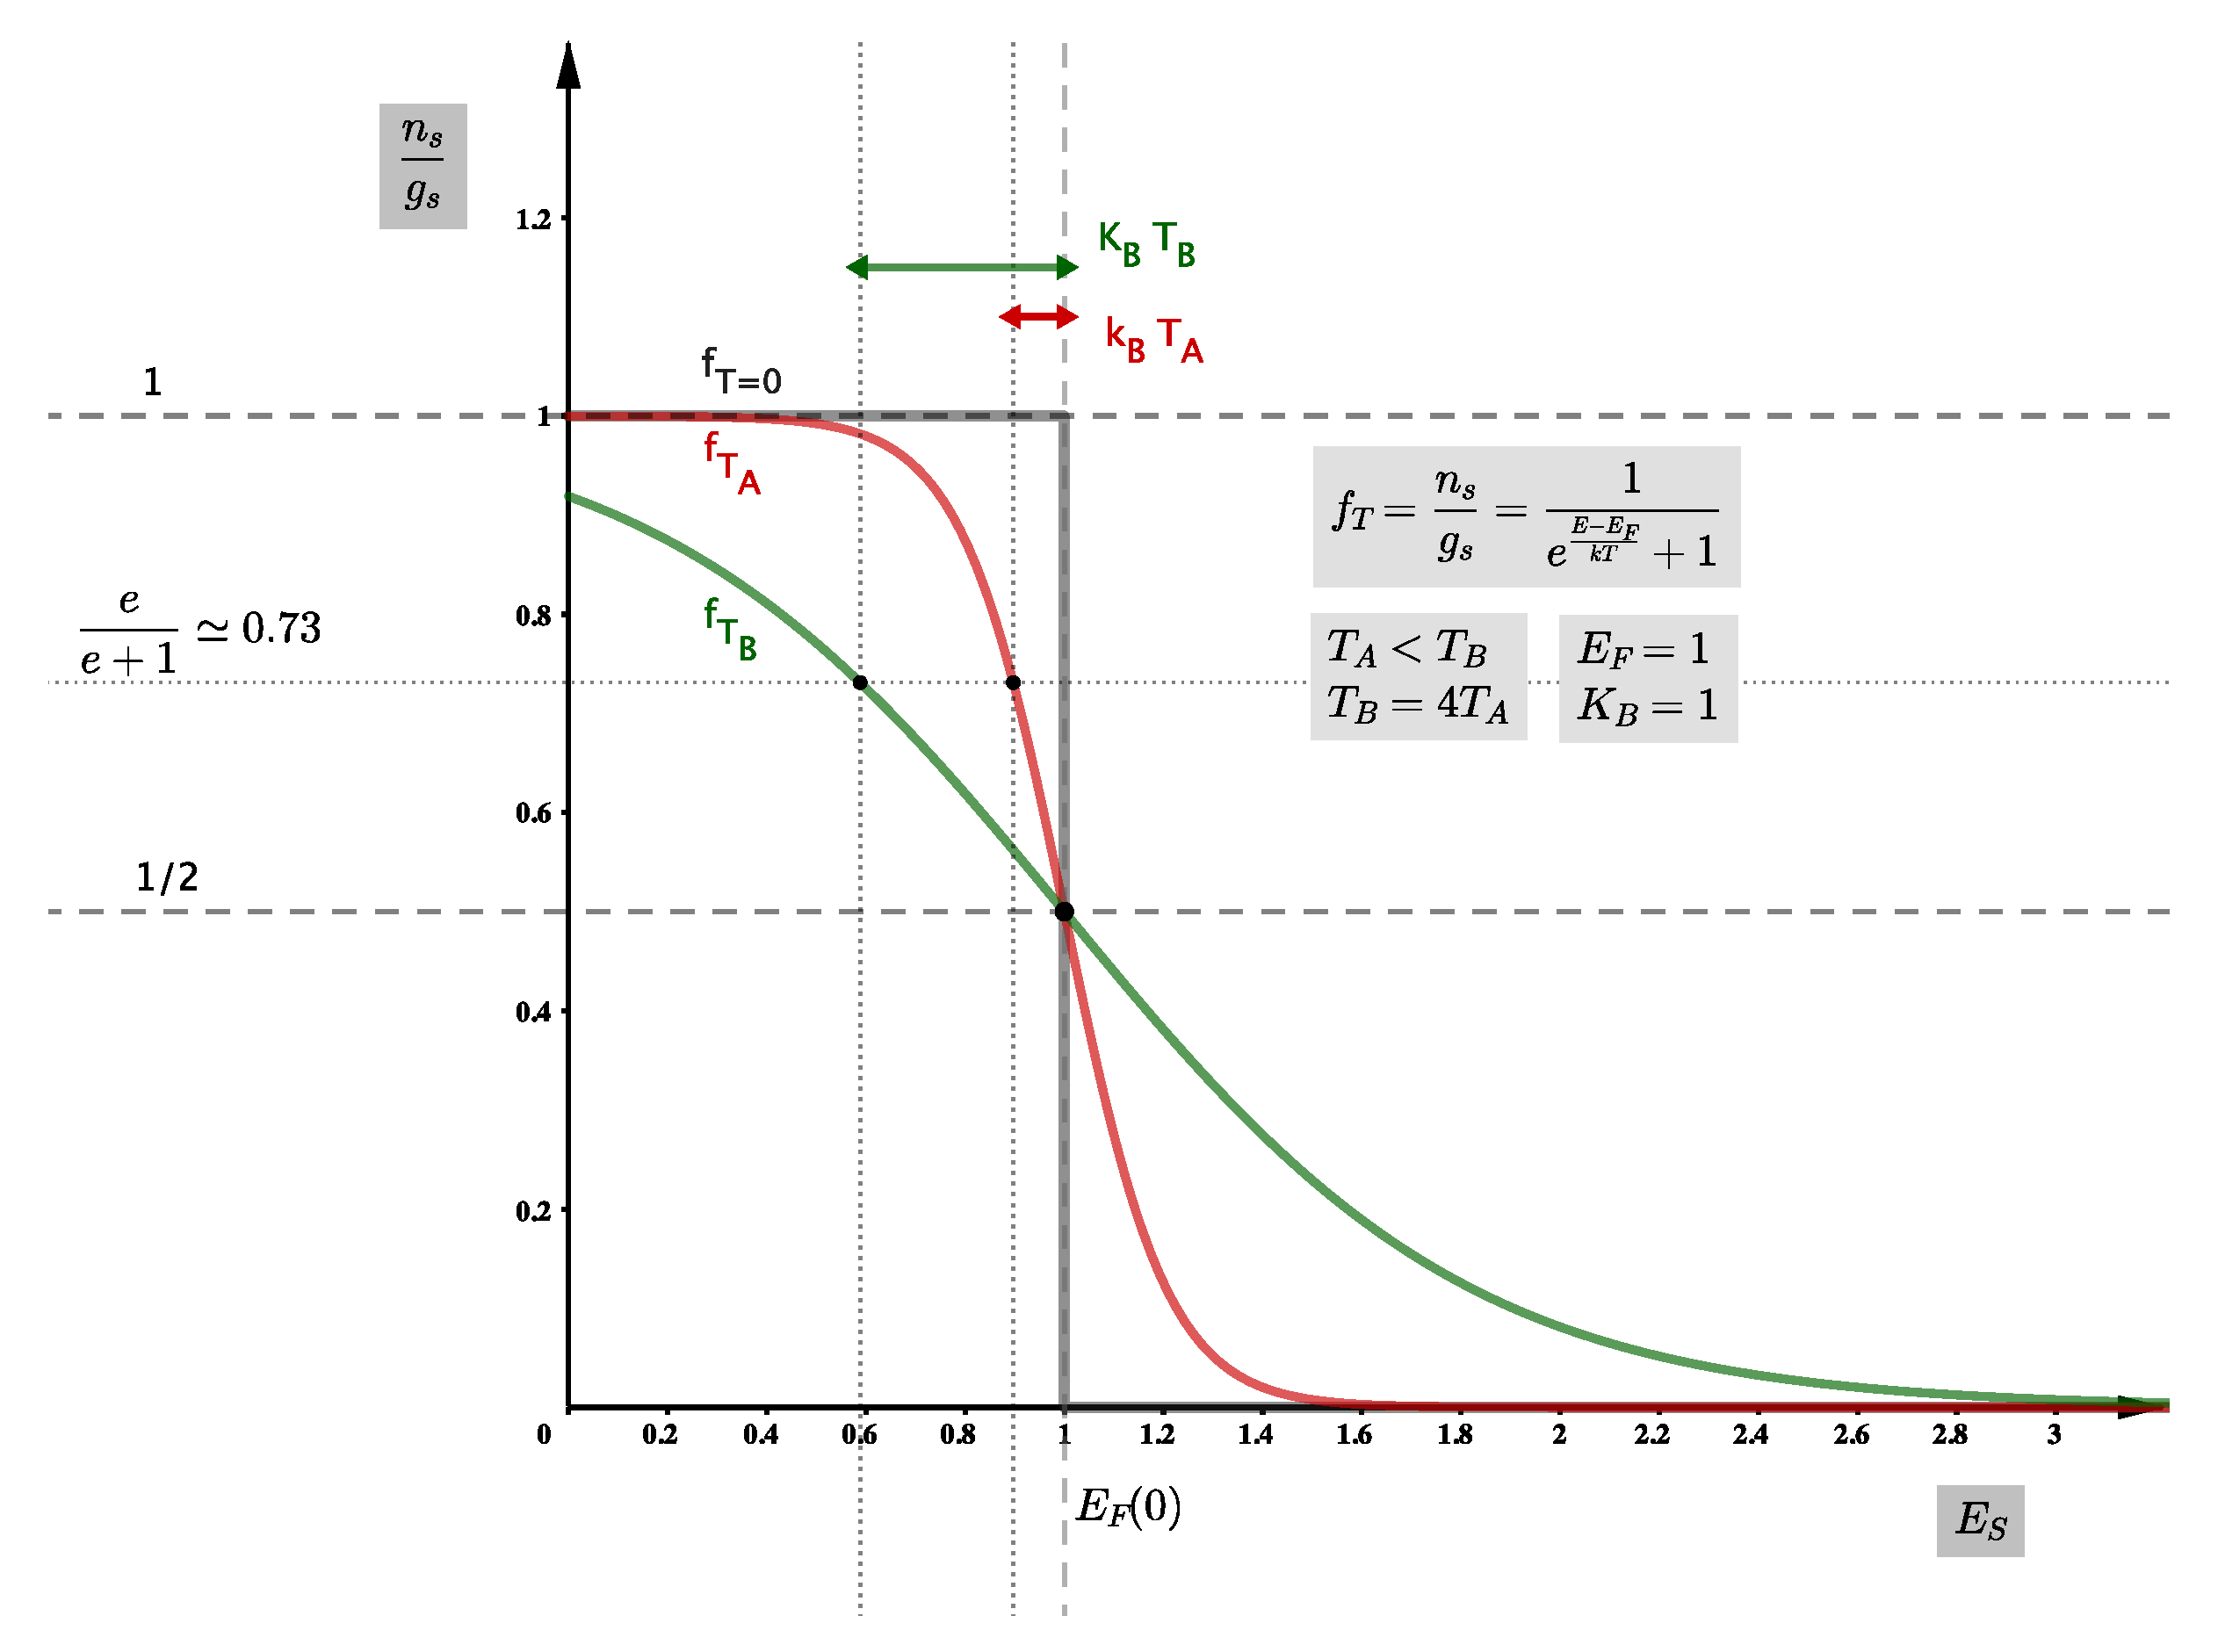
\includegraphics[scale=0.35]{/degenerazione3}
\label{grafico_distribuzioni}
\caption{Nel grafico vengono riportate tre distribuzioni calcolate su tre temperature, nel testo: \quad
Caso a) funzione $f_{T_A}$
Caso b) funzione $f_{T_B}$
Caso c) funzione $f_{T=0}$
}
\end{figure}

\subsection{Gas di elettroni}

Gli elettroni sono fermioni, la loro statistica è perciò descritta dal modello di Fermi-Dirac, poiché si tratta di particelle soggette al principio di esclusione di Pauli.
Gli \textbf{elettroni di conduzione nei metalli} sono un sistema quantistico anche a temperature \textit{normali} e non vicine allo zero assoluto, le densità tipiche di questi elettroni sono dell'ordine di $\SI{e28}{elettroni/m^3}$.

Quindi consideriamo un gas di elettroni, che seguono la statistica di Fermi Dirac, poiché fermioni, e si ha che la legge di distribuzione continua è la seguente, in cui compare $g(E)$ la \textit{funzione densità degli stati} (vedi \ref{fun_den_stat})
\begin{equation}
n(E)dE = \frac{ g(E)}{e^{ \frac{ E - E_F}{k_B T } } + 1 }
\quad\quad\quad\quad
g(E) = \frac{4 \pi V (2m^3)^{ \frac{1}{2} }}{h^3} E^{ \frac{1}{2} }
\end{equation}
trattandosi di elettroni, che hanno $spin=1/2$, gli stati disponibili raddoppiano e moltiplico x2, ottenendo
\begin{equation}
\begin{split}
n(E)dE & = 2 \cdot \frac{4 \pi V (2m^3)^{\frac{1}{2}} }{h^3} E^{\frac{1}{2}} \frac{1}{e^{\frac{E - E_F}{k_B T}} + 1} \\
& = \frac{8 \pi V (2m^3)^{\frac{1}{2}} E^{\frac{1}{2}}}{h^3} \frac{1}{e^{\frac{E - E_F}{k_B T}} + 1}
\label{nede_elet}
\end{split}
\end{equation}

\paragraph{Cerco l'espressione generale del Livello di Fermi}
Calcolo il numero totale delle particelle nel sistema, integrando in $[0, \infty]$
\begin{equation}
N = \int_0^{\infty} n(E)dE
\end{equation}
Se suppongo di essere alla temperatura dello \textit{zero assoluto} la temperatura è $T=0 K$ per cui la distribuzione è rappresentata dalla funzione a gradino ed allora ha senso calcolare l'integrale nell'intervallo $[0, E_F(0)]$ dove la distribuzione vale 1, oltre il valore $E_F(0)$ la distribuzione (il secondo fattore nella \ref{nede_elet}) vale 0.
Per cui equivale a calcolare il seguente integrale
\begin{equation}
\begin{split}
N & = \int_0^{E_F(0)} g(E)dE \\
& = \int_0^{E_F(0)} \frac{8 \pi V (2m^3)^{\frac{1}{2}} E^{\frac{1}{2}}}{h^3} dE \\
& = \frac{8 \pi V (2m^3)^{\frac{1}{2}}}{h^3} \int_0^{E_F(0)} E^{\frac{1}{2}} dE \\
\end{split}
\end{equation}






\newpage

\begin{equation}
N = \int_0^{\infty} n(E)dE = \int_0^{\infty} \frac{8 \pi V (2m^3)^{\frac{1}{2}} E^{\frac{1}{2}}}{h^3} \frac{ dE}{e^{ \frac{ E-E_F}{kT } } + 1 }
\end{equation}

Notiamo che allo zero assoluto si ha che 

\begin{equation}
\frac{ 1 }{e^{ \frac{ E - E_F}{kT } } + 1 } = 1 \quad
\mbox{come una funzione a gradino: } \quad
\begin{cases}
	1 \quad 0 \le E \le E_F \\
	0 \quad > E_F
\end{cases}
\end{equation}
dunque si semplifica scrivendo che 

\begin{equation}
\begin{split}
N = \int_0^{E_F(0)} g(E)dE & =  \int_0^{E_F(0)} \frac{8 \pi V (2m^3)^{\frac{1}{2}} E^{\frac{1}{2}}}{h^3} dE \\
& = \frac{16 \pi V (2m^3)^{\frac{1}{2}} }{3 h^3} [E_F(0)]^{\frac{3}{2}}
\end{split}
\end{equation}

\begin{equation}
\Longrightarrow \quad E_F(0) = \frac{ h^2}{8m } \Bigl(  \frac{ 3}{\pi } \frac{ N}{V }  \Bigr)^{ \frac{ 3}{ 2} } = \frac{ h^2}{8m } \Bigl(  \frac{ 3}{\pi } n \Bigr)^{ \frac{ 3}{ 2} }
\end{equation}

dove $n = \frac{ N}{V }$.
Da un punto di vista matematico si è calcolato l'area del sottografico come in figura

\begin{figure}[h]
\centering
\includegraphics[scale=0.07]{/gas_elettroni_areagrafico}
\caption{area grafico}
\end{figure}

Ad ogni modo si vede che il valore del livello di Fermi $E_F(0)$ aumenta all'aumentare del numero di particelle presenti nel sistema.
Calcoliamo quindi l'energia:

\begin{equation}
\begin{split}
U & = \int_0^{E_F(0)} E g(E)dE = \frac{8 \pi V (2m^3)^{\frac{1}{2}} }{h^3} \int_0^{E_F(0)} E^{ \frac{ 3}{2 } } dE \\
& = \frac{ 16}{5 } = \frac{ \pi V (2m)^{ \frac{ 1}{2 } }}{h^{ 3 } } \Bigl[ E_F(0) \Bigr]\frac{ 5}{2} \\
& = \frac{ 3}{2} N E_F(0)
\end{split}
\end{equation}


Dunque $\frac{ U}{N} = \frac{ 3}{5} E_F(0)$ e ciò significa che ogni particella, anche allo zero assoluto, 
possiede almeno un'energia minima pari a $\frac{ 3}{5} E_F(0)$, quindi anche per $T = 0 K $ si ha energia non nulla!
Come corollario si vede che il gas di fermioni, allo zero assoluto, possiede una pressione non nulla, detta
\underline{Pressione di Pauli}, pari a 

\begin{equation}
P = \frac{ 2}{3} \frac{ U}{N} = \frac{ 2}{5} n E_F(0)
\end{equation}

Poiché $\alpha = -\frac{ E_F}{k T} \quad \Rightarrow \quad \xi = e^{-\alpha} = e^{ \frac{ E_F}{k T}}$ allora si ha che per $T=0 \Rightarrow \xi = +\infty $
e si è in presenza di un gas totalmente degenere, che significa, nel caso di fermioni, che le particelle sono tutte "ammassate", pur rispettando il Principio di Esclusione di Pauli, nei livelli più bassi.
Un gas di fermioni continua a rimanere degenere se $T \ll T_F$ dove $T_F = \frac{ E_F(0)}{k}$, cioè se $kT \ll E_F(0)$, 
dove $E_F(T) \approx E_F(0)$ e quindi $\xi \gg 1$
In tal caso occorre usare la statistica di Fermi-Dirac.
Tuttavia se $kT \gg E_F(0) \Rightarrow T \gg T_F $, si deve (o si può?) applicare la statistica classica.

Supponiamo ora di avere un metallo di \underline{valenza 1} (la valenza esprime quanti elettroni di conduzione possono essere forniti da ogni atomo del metallo).
Supponiamo che la distanza fra gli elettroni sia $a \simeq \SI{0.1}{nm}$, allora una stima della densità elettronica è $n = \frac{ 1}{a^{ 3}} = a^{ -3}$.
Stimiamo $T_F$, perciò:

\begin{equation}
\begin{cases}
	T_F = \frac{ E_F(0)}{k} = \frac{ h^2}{8 k m} \Bigl(  \frac{ 3}{\pi}  \Bigr)^{ \frac{ 2}{3}} n^{ \frac{ 2}{3}} \simeq \frac{ h^2}{k m a^2} \simeq \frac{ 10^{ -68}}{10^{-23 } 10^{ 30} 10^{-20 }} \frac{ J \cdot s^2 \cdot K}{J \cdot Kg \cdot m^2} = 10^{5} K \\
	n^{ \frac{ 2}{3}} = \Bigl(  a^{ -3}  \Bigr)^{ \frac{ 2}{3}} = a^{ -2}
\end{cases}
\end{equation}

$T_F$ separa il regime di Fermi-Dirac da quello classico di Maxwell-Boltzmann, ed essendo dell'ordine di $10^{ -5}$, si ha che in situazioni ordinarie il sistema di elettroni è sempre degenere.
Il calcolo precedente è semplice perché si ha a che fare con lo zero assoluto, mentre le cose si complicano per $T \not = 0 $.

Studiamo ora la \underline{capacità termica} $C_V$, a volume costante: tale grandezza è legata a $T$ (temperatura assoluta).
Il contributo fondamentale alla capacità termica è dato dal reticolo del solido cristallino, ora studiamo il contributo elettronico.
Solo una frazione delle particelle vede variare la propria energia, perché siamo nel caso $T \not = o \ll T_F$, e tale variazione è:
$$ \Delta U \simeq N \frac{ k T}{E_F(0)} kT \simeq N\Bigl(  \frac{ T}{T_F}  \Bigr)kT $$

Poiché $C_V = \frac{ dU}{dT} \simeq N k \Bigl(  \frac{ T}{T_F}  \Bigr) $ usando $U = \frac{ 3}{2} N k T$ si ha che $C_V = \frac{ 3}{2} N k$ 
ed è allora necessario che $T$ sia confrontabile con $T_F \quad (T \approx T_F)$, ma ciò non accade nel caso ordinario per i fermioni,
per i quali quindi $C_V = C_V(T)$, e in particolare:
\begin{equation}
C_V = \frac{ \pi^2}{2} N k \Bigl(  \frac{ T}{T_F}  \Bigr)
\end{equation}

\begin{figure}[h]
\centering
\includegraphics[scale=0.1]{/buca_potenziale}
\caption{Buca di potenziale in un metallo}
\end{figure}

Consideriamo ora una \underline{buca di potenziale}: \\

Funzione lavoro $W_0 = h\nu_0 \Rightarrow V_0 = E_F(0) + W_0$ ed in generale si ha che $V_0$ è dell'ordine di qualche $eV$,
ad esempio l'argento ha $W_0 = \SI{4.7}{eV}$ e $ E_F(0) = \SI{5.5}{eV} $
Gli elettroni nel metallo riempiono i livelli energetici fino a $E_f(0)$. 
$W_0$ nei metalli è generalmente tale che $\SI{5}{eV} < V_0 < \SI{15}{eV} $

Questo spiega l'\underline{effetto termoionico}: è un fenomeno per cui un metallo riscaldato ad una temperatura sufficientemente alta inizia ad emettere elettroni presenti sulla sua superficie. A $T \not = 0 $ gli elettroni cominciano ad occupare gli strati più elevati e ad uscire dalla buca di potenziale.

















    
    %%
%% Author: dariochinelli
%% 2021-04-06
%%


\section{Calore specifico di un solido cristallino}
È stato un problema della fisica affrontato da molti studiosi, come Einstein e Debye, nel corso dei primi del '900, che ha aperto una nuova visione su vari ambiti.
il calore specifico molare a volume costante è definito come
\begin{equation}
c_V = \frac{1}{N} \frac{dU}{dT}
\end{equation}
dove $N$ rappresenta il numero di moli.
Questa grandezza misura l'energia necessaria per far variare di un grado la temperatura di una mole di sostanza.
Un cristallo è una struttura geometrica in cui gli atomi occupano posizioni ben precise.
Quindi studiamo il calore specifico di un reticolo tridimensionale di atomi.
In Fisica classica il calore specifico di un solido è lo stesso per tutti i materiali, in una mole ci sono $N_A$ atomi ed ognuno di questi atomi può eseguire oscillazioni armoniche semplici attorno alla posizione di equilibrio, da cui si scrive l'energia totale considerando le tre dimensioni come
\begin{equation}
U = 3 N_A k_B T = 3 R T
\end{equation}
in cui ogni oscillatore armonico ha una energia media $k_B T$, come calcolato anche grazie alla statistica classica di Maxwell Boltzmann nei capitoli precedenti, 
ed in cui $R$ è la costante universale dei gas.
Eseguendo la derivata ottengo la \textbf{legge classica di Dulong Petit (1819)}
\begin{equation}
c_V = \frac{dU}{dT} = 3 R = \SI{6}{cal / mol . K}
\end{equation}




\newpage


Il calore specifico di una sostanza esprime infatti il modo in cui tali atomi riescono nelle loro posizioni reticolari.

In una mole ci sono un numero di Avogadro di atomi, e ogni atomo può essere visto come un punto materiale che compie semplici oscillazioni armoniche, per cui,
considerando lo spazio tridimensionale, una mole di sostanza solida ha $3 N_a$ gradi di libertà.

A ogni grado di libertà, in accordo con la legge di Equipartizione dell'energia, è assegnata una energia totale media $kT$, dunque:

\begin{equation}
U = 3 N_a k T = 3 R T
\end{equation}
\begin{figure}[h]
\centering
\includegraphics[scale=0.08]{/andamento_Cv}
\caption{andamento di $C_V$}
\end{figure}
Dove $R$ è la costante universale dei gas. 
Perciò si ha che $C_V = 3 R \simeq \SI{6}{cal / (mol * K)}$ che è la \underline{Legge di Dulong-Petit}, scoperta nel 1819, che afferma che i solidi hanno un calore specifico costante. 
Tuttavia sperimentalmente si osservò che tutto questo valeva solo a temperature elevate.
Nelle vicinanze dello zero assoluto invece il calore specifico tende a zero e a basse temperature ha un andamento del tipo $C_V \propto T^3$.

Fu Einstein a cercare di proporre un modello teorico che fosse più consistente con l'evidenza sperimentale nel 1905.
Egli ritenne che ad ogni mole di sostanza non si dovesse associare un'energia $kT$ bensì un termine che tenesse conto della quantizzazione.
Esattamente come fece Planck per il Corpo Nero, Einstein considerò che ogni mole di sostanza avesse un'energia data dal termine
$$E = \frac{ h \nu}{e^{ \frac{ h\nu}{k T } } - 1 }$$, 
pensando che il sistema non fosse altro che un insieme di $3 N_A$ oscillatori armonici semplici, aventi tutti la stessa frequenza di oscillazione.
Dunque per $n=1$:

\begin{equation}
\begin{cases}
	U = 3 N_A \frac{ h \nu}{e^{ \frac{ h \nu}{ k T} } - 1 } \\
	\beta = (k T)^{ -1 }
\end{cases}
\Rightarrow \quad C_V = \frac{ dU}{dT } = \frac{ 3 N_A}{k T^2 } (h \nu)^2 \frac{ e^{ \beta h \nu }}{\Bigl(  e^{ \beta h \nu } - 1   \Bigr)^2}
\end{equation}

Per temperature elevate, dunque per $\beta \sim 0$, si può esprimere l'esponenziale $e^{ \beta h \nu } = 1 + \beta h \nu + ...$
da cui $U(\beta \sim 0) = \frac{ 3 N_A h \nu}{\beta h \nu } = 3 N_A k T = 3 R T$ come avevano trovato Dulong e Petit.

Mentre nel caso di $k T \leq h \nu$ si nota che $C_V$ cala in quanto l'energia termica diventa confrontabile con la distanza fra i livelli energetici e dunque diventa rilevante la quantizzazione dell'energia.
In particolare per $k T \ll h \nu$ si ha che $\Bigl(  e^{ \beta h \nu } - 1  \Bigr) \sim e^{ \beta h \nu }$, perciò si ottiene, in accordo con l'evidenza sperimentale, che:

\begin{equation}
C_V = \frac{ 3 N_A (h \nu)^2}{k T^2 }e^{ - \beta h \nu } \quad \Rightarrow \quad \lim_{T \to 0} C_V = 0
\end{equation}

Dunque il modello di Einstein fu un notevole passo avanti, ma rimaneva ancora un problema: non si adattava, a basse energie, l'andamento come $T^3$ del calore specifico.
Ciò è da ricondurre ad un errore nelle assunzioni di Einstein: non c'era alcun motivo per cui le frequenze degli oscillatori armonici dovessero essere le stesse, anche perché questo avrebbe implicato l'esistenza di una frequenza caratteristica diversa per ogni materiale, ipotesi priva di fondamento.
A risolvere questi interrogativi fu Debye col suo modello nel 1912, che considerò come gli $N$ atomi avessero, in una mole di sostanza, un moto collettivo.
Il moto generale degli $N_A$ atomi è rappresentato dalla combinazione lineare di $3N_A$ modi di vibrazione ($N_A$ nel caso 1-D), ognuno avente una propria frequenza $\nu$.
A partire da questo sistema, Debye lo semplificò ulteriormente, pensando al solido come un sistema continuo.
Fece l'approssimazione di considerare onde longitudinali aventi il vincolo di avere nodi ai bordi del sistema.
Questo calcolo condusse ad un risultato quasi uguale a quello del Corpo Nero:

\begin{equation}
N(\nu)d\nu = \frac{ 4 \pi V}{v^3 } \nu^3 d\nu
\end{equation}

Dove si 4 al posto di 8 perché le onde elettromagnetiche sono anche trasversali e ovviamente si ha che $v \not = c$.
Tuttavia il sistema non è in verità continuo bensì discreto, per cui, per tenerne conto, Debye impose che:

\begin{equation}
\begin{split}
& \int_0^{\nu_m} N(\nu)d\nu = 3 N_A \quad \quad \mbox{dove $\nu_m$ è una \underline{frequenza di taglio}} \\
& \int_0^{\nu_m} \frac{ 4 \pi V}{v^3 } \nu^3 d\nu = 3 N_A \Rightarrow \frac{ 4 \pi V}{3 v^3 } \nu_m^3 = 3N_A \Rightarrow \nu_m = \Bigl(  \frac{ 3 N_A}{4 \pi V }  \Bigr)^{ \frac{ 1}{3 } }
\end{split}
\end{equation}

Ad ogni oscillatore viene associata una energia media $\varepsilon = \frac{ h \nu}{e^{ \frac{ h \nu}{k T } } - 1 }$, da cui si ottiene che:

\begin{equation}
\begin{split}
U & = \int_0^{\nu_m}  \frac{ h \nu}{e^{ \frac{ h \nu}{k T } } - 1 } \frac{ 4 \pi V}{v^3 } \nu^3  d\nu \quad \Rightarrow \quad
\begin{cases}
	\mbox{pongo:} \quad x \frac{ h \nu}{k T } \Rightarrow x_m = \frac{ h \nu_m}{k T } \\
	d\nu = \frac{ kT}{h } dx
\end{cases} \\
& = \frac{ 4 \pi V}{v^3 } \Bigl(  \frac{ kT}{h }  \Bigr)^4 h \int_0^{x_m} \frac{ x^3 dx}{e^x -1 } \\
& = \frac{ 9 R T}{x_m^3 } \int_0^{x_m} \frac{ x^3 dx}{e^x - 1 } \\
& = \frac{ 9 R T^4}{\Theta^3 } \int_0^{\Theta / T} \frac{ x^3 dx}{e^x -1 } \quad \mbox{con: } x_m = \frac{ \Theta}{T }
\end{split}
\end{equation}

Allora:
\begin{equation}
C_V = \frac{ dU}{dT } = 9R \Bigl[ 4 \Bigl(  \frac{ T}{\Theta }  \Bigr)^3 \int_0^{\Theta / T} \frac{ x^3 dx}{e^x -1 } - \frac{ \Theta}{T }\frac{ 1}{e^{ \frac{ \Theta}{T } } - 1 } \Bigr]
\end{equation}

Dunque:
\begin{equation}
\Theta = \frac{ h}{k } \Bigl(  \frac{ 9N_A}{4 \pi V }  \Bigr)^{ \frac{ 1}{3 } } v
\end{equation}
è una temperatura oltre la quale tutti i modi di vibrazione sono attivi.

Vediamo la $\Theta$ di alcuni materiali:
\begin{table}[h]
\centering
\begin{tabular}{|l|l|}
\hline
\textbf{Sostanza}    & \textbf{$\Theta$} \\ \hline
Elio solido & 30 K     \\ \hline
Ferro       & 465 K    \\ \hline
Diamante    & 1860 K   \\ \hline
\end{tabular}
\end{table}


\begin{equation}
\begin{split}
& \mbox{Se} \quad T \ll \Theta \Rightarrow \frac{ \Theta}{T } \sim \infty \Rightarrow 9R \frac{ T^4}{\Theta^3} \int_0^{\infty} \frac{ x^3 dx}{e^x - 1} = \frac{ 3}{5 } \pi^4 R \Bigl(  \frac{ T^4}{ \Theta^3}  \Bigr) \\
& \Rightarrow C_V = \frac{ 12}{5 } \pi^4 R \Bigl(  \frac{ T}{\Theta }  \Bigr)^3 \quad \mbox{ed ecco l'attesa dipendenza da $T^3$} \\
& \mbox{Se} \quad T \gg \Theta \mbox{, si ha che} \quad e^x = 1 + x + ... \quad (x \sim 0) \\
& \Rightarrow U = \frac{ 9R T^4}{\Theta^3 } \int_0^{\frac{ \Theta}{ T}} \frac{ x^3}{x }dx = \frac{ 9 R T^4}{3 \Theta^3 } \frac{ \Theta^3}{T^3 } = 3RT \quad \mbox{Come scoperto da Dulong-Petit}
\end{split}
\end{equation}
Il modello di Debye è semplice ma grazie alle sue assunzioni fornisce, per usando la statistica di Maxwell-Boltzmann, risultati eccellenti.
È lecito usare la statistica classica in quanto i modi sono distinguibili nel reticolo cristallino.
Occorre fare delle considerazioni sui contributi a $C_V$:

\begin{equation}
\begin{cases}
	\mbox{Contributo reticolare} \quad C_V = \frac{ 12}{5 } \pi^4 R \Bigl(  \frac{ T}{\Theta }  \Bigr)^3 \\
	\mbox{Contributo elettronico} \quad C_V = \frac{ \pi^2}{2 } N k \Bigl(  \frac{ T}{T_F}  \Bigr) \\
\end{cases}
\Rightarrow \frac{ C_{VR}}{C_{VE} } = \frac{ 5}{24 \pi^2 }\frac{ N}{N_A } \frac{ \Theta^3}{T^2 T_F } \Rightarrow T_0 \simeq \Bigl(  \frac{ \Theta}{T_F }  \Bigr)^{ \frac{ 1}{2 } } \Theta
\end{equation}
Oltre la temperatura $T_0$ il contributo reticolare è maggiore di quello elettronico.
Quello elettronico supera quello reticolare solo quando si è vicini allo zero assoluto per i metalli, dove ci si aspetta quindi un andamento lineare. 



























    
    %%
%% Author: dariochinelli
%% 2021-04-07
%%


\section{Catena unidimensionale di atomi (\textit{dinamica fononica})}
Per questo studio considero una catena unidimensionale, che non è il problema più generale in tre dimensioni da poter risolvere ma generalizza meglio il problema visto nel capitolo precedente sullo studio approssimato di Debye. \\

% ------- ------- ------- ------- ------- ------- ------- ------- ------- ------- -------
Un mezzo solido continuo supporta sia vibrazioni longitudinali sia trasversali, ma Debye ha agito nel modo seguente:
\begin{equation}
\int_0^{\nu_m} N(\nu) d\nu = 3 N_A \Rightarrow \frac{ 4\pi V}{v^3 } \nu_m^3 = 3 N_A
\end{equation}
Ma nel caso più corretto possibile, il solido in questione, soffre di oscillazioni sia trasversali che longitudinali.
Occorre dunque dividere la velocità dell'onda nelle sue componenti.
\begin{equation}
3N_A = \frac{ 3 \pi V}{3 } \nu_m^3 \Bigl(  \frac{ 1}{v_l^3 } + \frac{ 2}{v_t^3 }  \Bigr) \quad\quad \mbox{dove si è usato} \quad
\frac{ 1}{v^3 } = \Bigl(  \frac{ 1}{v_l^3 } + \frac{ 2}{v_t^3 }  \Bigr)
\end{equation}
Dove il 2 sta ad indicare che le onde trasversali hanno due possibili stati di polarizzazione, mentre ce n'è uno solo per le onde longitudinali,
e dunque ciò che abbiamo visto finora vale solo nel caso in cui le onde sono tutte longitudinali, ma ciò non è sempre vero. \\
% ------- ------- ------- ------- ------- ------- ------- ------- ------- ------- -------

Consideriamo quindi una catena unidimensionale di atomi chiusa su se stessa, a \textit{collana}, e detta condizione al contorno di Born–von Karman e cerco di calcolare il numero di modi di vibrazione.
Introduciamo la seguente nomenclatura:
\begin{equation}
\begin{split}
x_n & = \mbox{ posizione $n$-esima particella} \\
R_n & = \mbox{ posizione di equilibrio $n$-esima particella} \\
u_n & = (x_n - R_n) = \mbox{ spostamento dalla posizione di equilibrio } \\
a & = \mbox{ distanza reticolare, distanza fra due posizioni di equilibrio} \\
K & = \mbox{ costante elastica delle molle} \\
\end{split}
\end{equation}
\begin{figure}[h]
\centering
\includegraphics[scale=0.2]{/catena_unidim_atomi}
\caption{Catena unidimensionale di atomi}
\end{figure}
Poiché la catena è chiusa, si impongono condizioni al contorno periodiche.
La forza di interazione tra due particelle è nulla quando la molla è all'equilibrio e cioè quando $x_2-x_1 = a$, quando si trovano ad una distanza $a$, quindi la forza $F_{21}$ che agisce sulla particella $2$ a causa della connessione con $1$
\begin{equation}
\begin{split}
F_{21} & = - K (x_2 - x_1 - a) \\
& = - K (x_2 - R_2 - x_1 + R_1 + R_2 - R_1 - a) \\
& = - K (u_2 - u_1)
\end{split}
\label{forza_F21}
\end{equation}
L'equazione del moto è data da due termini: uno ricavato sopra \ref{forza_F21} ed uno analogo tra la particella $2$ e la particella $3$
\begin{equation}
m \ddot{x_2} = - K (u_2 - u_1) + K (u_3 - u_2)
\end{equation}
la somma è dovuta al fatto che quando la quantità al secondo membro è positiva, l'interazione spinge la particella verso destra sull'asse $x$.
Le derivate seconde $\ddot{x_2} = \ddot{u_2}$ sono equivalenti, per cui è dunque possibile scrivere l'equazione del moto generica per l'$n$-esima particella, 
(sulla quale però si approssima valutando solo le interazioni fra le particelle adiacenti)
\begin{equation}
\begin{split}
m \ddot{u_n} & = - K (u_n - u_{n-1}) + K (u_{n+1} - u_n) \\
& = K \Bigl[  u_{n-1} + u_{n+1} - 2 u_n  \Bigr]
\label{eqmoto_nesimapart}
\end{split}
\end{equation}
La soluzione di questa equazione può essere espressa come onda longitudinale \textit{viaggiante} del tipo
\begin{equation}
u_n = s e^{ i k R_n } e^{ - i \omega t } = s e^{ i (k n a - \omega t) }
\label{solution_un}
\end{equation}
dove
\begin{equation}
\begin{split}
k = \frac{2\pi}{\lambda} \quad \mbox{numero d'onda} \quad\quad&\quad\quad s  = \quad \mbox{ampiezza} \\
\omega = 2 \pi \nu  \quad \mbox{frequenza} \quad\quad\quad\quad&\quad\quad R_n = n a \\
\end{split}
\end{equation}
Sostituendo la soluzione \ref{solution_un} nell'equazione differenziale \ref{eqmoto_nesimapart} dopo aver trovato la derivata 
\begin{equation}
\frac{d^2}{dt^2} u_n = \ddot{u_n} = -\omega^2 s e^{ i ( k n a - \omega t ) }
\end{equation}
ottengo
\begin{equation}
\begin{split}
- \omega^2 m s e^{ i (k n a - \omega t) } & = K \Bigl(  s e^{ - i \omega t }  \Bigr) \Bigl[  e^{ i k (n-1) } + e^{ i k (n+1) } - 2 e^{ i k n } \Bigr] \\
- \omega^2 m s e^{ i k n a } & = K \Bigl[  e^{ - i k a } + e^{ i k a } - 2 \Bigr] e^{ i k n a } \\
\omega^2 m  & = K ( 2 - 2 \cos (k a) )
\end{split}
\end{equation}
utilizzo l'identità trigonometrica: $\sin^2 \frac{ X}{2 } = \frac{ 1}{2 } \Bigl(   1 - \cos(X)  \Bigr)$
\begin{equation}
\omega^2 = \frac{4 K}{m} \sin^2 \frac{k a}{2} 
\quad\Rightarrow\quad 
\omega = 2 \sqrt{\frac{K}{m}} \Bigl| \sin \frac{ka}{2}  \Bigr| \quad\quad\quad \mbox{(da ricordare)}
\label{omega}
\end{equation}
questa formula collega insieme la frequenza $\omega$ ed il numero d'onda $k$.

\paragraph{Studio la funzione in base al valore di $k$} 
Per piccoli numeri d'onda $k$, cioè per grandi lunghezze d'onda $\lambda$, posso approssimare la \ref{omega} con
\begin{equation}
\omega = 2 \sqrt{\frac{K}{m}} \Bigl| \frac{ka}{2}  \Bigr|  \quad\Rightarrow\quad \omega \propto k
\end{equation}
per cui la \textit{velocità di fase}
\begin{equation}
v_{fase} = \frac{\omega}{k}
\end{equation}
è uguale alla \textit{velocità di gruppo}
\begin{equation}
v_{gruppo} = \frac{d \omega}{d k}
\end{equation}
da cui trovo che è indipendente dalla frequenza e vale
\begin{equation}
\frac{\omega}{k} = c = \frac{d \omega}{d k} = \sqrt{\frac{K}{m} a^2}
\end{equation}
allora si dice che \textit{non c'è dispersione}.

Per valori qualsiasi di $k$, uso la \ref{omega} e trovo la funzione $\sin$, periodica su un periodo $2\pi / a$.
La funzione \ref{omega} nell'intervallo $\Bigl[  -\frac{\pi}{a}, +\frac{\pi}{a}  \Bigr]$, detta \textit{"1st Brillouin Zone"}, plottata permette di capire meglio il concetto di dispersione, vedi figura \ref{dispersione} \\
\begin{figure}[h]
\centering
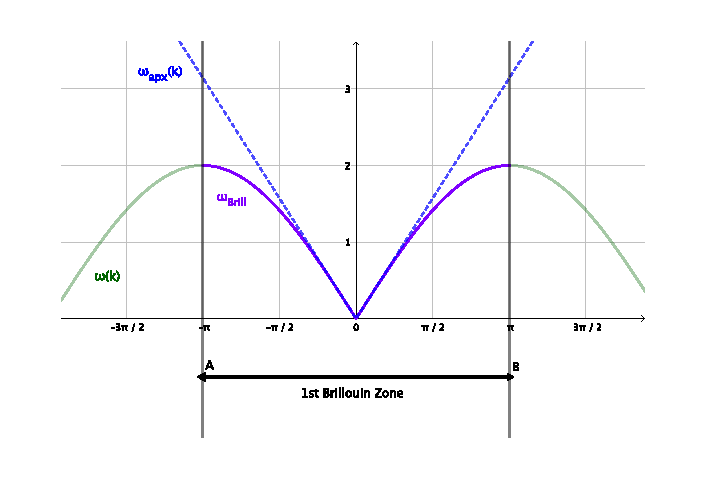
\includegraphics[scale=0.8]{/brillouinzone}
\caption{Curva di dispersione, zona di Brillouin}
\label{dispersione}
\end{figure}
Il distacco tra la funzione lineare e la funzione seno è dovuto al fatto che non ho a che fare con un sistema continuo ma discreto.
Per piccoli $k$ per cui le due curve combaciano, non ho dispersione, mentre per $k$ più grandi le due curve si allontanano e ho dispersione.
Cioè aumentando $k$ non è più vero che la velocità non dipende dalla frequenza e quindi avrò onde a diverse velocità, quindi dispersione.

\paragraph{Condizioni su $k$} avendo considerato una catena di atomi circolare, si dovrà imporre l'uguaglianza tra la funzione relativa al primo atomo e quella relativa all'atomo $N+1$ ovvero
\begin{equation}
\begin{split}
u_1 &= u_{N+1} \\
s \Bigl(  e^{ ika } e^{ -i \omega t }  \Bigr) & =  s \Bigl(  e^{ ik(N+1)a } e^{ -i \omega t }  \Bigr) = s \Bigl(  e^{ ika } e^{ ikNa } e^{ -i \omega t }  \Bigr)
\end{split}
\end{equation}
vera se soddisfa la condizione 
\begin{equation}
e^{ ikNa } = 1
\end{equation}
ovvero
\begin{equation}
k = \frac{2\pi}{N a} l \quad\quad\quad \mbox{quindi} \quad -\frac{N}{2} < l \le \frac{N}{2}
\end{equation}
quindi se $k$ varia di una quantità $\frac{2\pi}{a}$ allora $u_n$ non cambia;
ci sono allora solo $N$ valori di $k$ consistenti con la condizione scritta sopra.


\subsection{Fononi}
In alternativa alla trattazione del capitolo precedente, posso ragionare in termini di particelle per cui ho un modo di frequenza $\omega(k)$ con energia
\begin{equation}
\varepsilon = n h \nu = n \hbar \omega
\end{equation}
e considerare lo stato che contiene $n$ particelle con energia $\hbar \omega$ e numero d'onda $k$
\begin{equation}
\bar \varepsilon = \frac{h \nu}{e^{ \frac{h\nu}{k_B T} } - 1}  
= \frac{\hbar \omega}{e^{ \frac{\hbar\omega}{k_B T} } - 1}  
\end{equation}
tali particelle sono dette \textit{fononi}, descrivibili come i quanti di energia elastica (meccanica), collegata ai moti di vibrazione reticolare.
Sono definite come particelle a \textit{massa nulla} e \textit{spin zero}, sono quindi descrivibili come \textit{bosoni}.
Si può vedere come l'analogo di un fotone: quanto di energia elettromagnetica, ma relativo alle onde elastiche. \\
Utilizzando i \textit{fononi} è possibile trattare alcuni fenomeni di fisica classica e dello stato solido come ad esempio:
\begin{itemize}
\item il calore specifico
\item la resistenza elettrica
\item la trasmissione del calore attraverso un metallo
\item la misura di diffrazione neutronica
\end{itemize}





    
    %%
%% Author: dariochinelli
%% 2021-01-25
%%

\section{Applicazione della statistica di Bose-Einstein al Corpo Nero}

Oltre alla possibilità di utilizzare la statistica di Maxwell-Boltzmann per risolvere il problema del Corpo Nero, come già affrontato,
un altro modo di affrontare il problema è considerare che la luce, nella cavità di Corpo Nero, sia un gas di fotoni, che sono bosoni.
Per queste particelle occorre usare la statistica di Bose-Einstein,
\begin{equation}
\frac{ n_s}{g_s } = \frac{ 1}{e^{ \alpha + \beta E_s } - 1 }
\end{equation}
poiché si tratta di bosoni, i fotoni non sono soggetti al Principio di Esclusione di Pauli, e quindi tendono ad accumularsi nel livello energetico più basso,
quello fondamentale $E=0$, avente energia minore.
Nel caso di fotoni, $\alpha = 0$ poiché il numero di particelle nel sistema non si cQUALCOSA necessariamente.
Infatti all'interno della cavità di Corpo Nero c'è uno scambio continuo fra il campo di radiazione e le pareti della cavità: $e^{ alpha } = 1 \Rightarrow \xi = 1$.
Dunque un gas di fotoni è sempre degenere.
Ogni modo di vibrazione può essere considerato come uno stato energetico occupato da $n$ fotoni, ciascuno con energia $h \nu$.
Calcoliamo dunque la radianza:

\begin{equation}
\begin{split}
& E_s = h \nu \quad \quad \beta = (kT)^{ -1 } \\
& n_s = \frac{ g_s}{e^{ \beta E_s } - 1 } \Rightarrow \bar \varepsilon = \frac{ E_s}{e^{\beta E_s } - 1 } \\
& g(\nu) d\nu = N(\nu)d\nu = \frac{ 8 \pi V}{c^3 } \nu^3 d\nu
\end{split}
\end{equation}

\begin{equation}
\begin{split}
\epsilon_T(\nu) d\nu & = \frac{ 1}{V } (h\nu) \frac{ 8 \pi V}{c^3 }d\nu \frac{ 1}{e^{ \frac{ h\nu}{kT } } - 1 }\nu^2 \\
& = \frac{ (h\nu) 8 \pi}{c^3} \nu^2 \frac{ 1}{e^{ \frac{ h\nu}{kT } } - 1 }
\end{split}
\end{equation}

Siamo dunque pervenuti allo stesso risultato di Planck, pur utilizzando la statistica di Bose-Einstein anziché quella classica.

Si può eseguire il conto esprimendo $g=g(E)$, da cui:
\begin{equation}
\begin{split}
n(E)dE & = \frac{ g(E) dE}{e^{ \beta E } - 1 } \\
g(\nu) d\nu & = \frac{ 8 \pi V}{c^3 } \nu^2 d\nu \Rightarrow g(E) = \frac{ 8 \pi V}{c^3 } \frac{ E^2 dE}{h^3 } \\
& \begin{cases}
	E = h\nu \Rightarrow \nu = \frac{ E}{h } \\
	d\nu = \frac{ dE}{h }
\end{cases} \\
\epsilon_T(E)dE & = \frac{ E}{V } n(E) dE = \frac{ 8\pi E^3 dE}{c^3 h^3 (e^{ \beta E } - 1) }
\end{split}
\end{equation}
Debye assunse che ogni modo di vibrazione altro non fosse che un oscillatore semplice avente energia
$$E=n \hbar \omega \Rightarrow \bar \varepsilon = \frac{ \hbar \omega}{e^{ \frac{ \hbar \omega}{ kT} } - 1 }$$
Difatti ogni modo di vibrazione è uno stato che contiene un numero $N$ di \underline{fononi}, entità analoghe ai fotoni.
Un fonone è il quanto di energia vibrazionale del sistema, esattamente come il fotone è il quanto di energia elettromagnetica.
I fotoni, quasi-particelle prive di massa, possono quindi essere trattati come bosoni (hanno spin $= 0$ e $\alpha = 0$), e si può applicare la statistica di Bose-Einstein.











    
    %%
%% Author: dariochinelli
%% 2021-04-08
%%


\subsection{Condensazione di Bose-Einstein}
Considero un gas di bosoni, la statistica che lo regola è 
\begin{equation}
\frac{n_s}{g_s} = \frac{1}{e^{ \alpha + \beta E_s } - 1}
\end{equation}
ed imponendo che i parametri di Lagrange siano
\begin{equation}
\beta = \frac{1}{k_B T} \quad\quad\quad \alpha > 0
\end{equation}
trovo che a temperatura $T = \SI{0}{K}$ solo gli stati con $E_s = 0$ sono occupati, assumendo $g_0  = 1$ trovo
\begin{equation}
N \simeq \frac{ 1}{e^{ \alpha } - 1 }
\label{N_alpha}
\end{equation}
ed invertendo trovo la relazione
\begin{equation}
e^{\alpha} = 1 + \frac{1}{N} \simeq 1 \quad \mbox{quando } N \to \infty
\end{equation}
per cui il sistema è degenere.
Essendo $\alpha \to 0$ posso sviluppare la \ref{N_alpha} come
\begin{equation}
N \simeq \frac{1}{1+ \alpha - 1} = \frac{1}{\alpha}
\end{equation}
lasciando esplicito $g_0$ avrei
\begin{equation}
n_0 \simeq N \simeq \frac{g_0}{e^{ \alpha } - 1 }
\quad\quad
e^{\alpha} = 1 + \frac{g_0}{N} \simeq 1
\quad\quad
N \simeq \frac{g_0}{\alpha}
\end{equation}

La relazione 
\begin{equation}
e^{\alpha} \simeq 1
\end{equation}
resta valida anche a $T \not= 0$ vicina allo zero assoluto, per cui posso chiedermi quante particelle sono all'energia \emph{ground state} $E_s = 0$?
Cerco un'espressione per $n_0$, il ground state, in funzione della temperatura
\begin{equation}
N = \sum_s n_s = n_0 (T) + n_e(T)
\end{equation}
ovvero la somma tra il numero di particelle nello stato fondamentale più il numero di particelle in tutti gli altri stati, stati eccitati.
Utilizzo l'equazione al continuo per la legge di Bose Einstein e la funzione densità degli stati 
\begin{equation}
\begin{split}
n(E)dE & = g(E) \frac{ 1}{e^{ \alpha + E / k_B T } - 1 } dE \\
g(E)dE & = \frac{4\pi V (2m^3)^{ \frac{1}{2} }}{h^3} E^{ \frac{1}{2} } dE
\end{split}
\end{equation}
e quindi integro nell'intervallo $\Bigl[  0, \infty  \Bigr]$
\begin{equation}
\begin{split}
N & = n_0 + \int_0^{\infty} n(E)dE \\
& = n_0 + c \int_0^{\infty} \frac{E^{ \frac{1}{2} }}{e^{ \alpha + \beta E } - 1} dE
\end{split}
\end{equation}
in cui ho sostituito e sostituisco
\begin{equation}
\begin{split}
& c = \frac{4\pi V (2m^3)^{ \frac{1}{2} }}{h^3} \\
& z= \beta E \quad\quad\quad dE = \frac{dz}{\beta} = dz k_B T
\end{split}
\end{equation}
e ottengo
\begin{equation}
N = n_0 + c(k_B T)^{\frac{3}{2}} G(\alpha)
\label{N_di_gamma}
\end{equation}
definendo la funzione \emph{gamma}
\begin{equation}
G(\alpha) = \int_0^{\infty} x^{ \frac{1}{2} } (e^{ z + \alpha } - 1) dz
\end{equation}
Se $\alpha$ è grande
\begin{equation}
\begin{split}
G(\alpha) & = e^{ - \alpha} \int_0^{\infty} x^{ \frac{1}{2} } e^{ -z } dz \\
G(\alpha) & \to e^{-\alpha} \frac{\sqrt{\pi}}{2}
\end{split}
\end{equation}
Se $\alpha$ è piccolo
\begin{equation}
\begin{split}
& G(0) \to 2.612 \frac{\sqrt{\pi}}{2} \\
& \alpha \simeq \frac{1}{N} \to 0 \quad\Rightarrow\quad G(\alpha) \approx G(0)
\end{split}
\end{equation}
allora l'equazione \ref{N_di_gamma} diventa
\begin{equation}
\begin{split}
N = n_0 + c (k_B T)^{ \frac{3}{2} } G(\alpha)
\quad\Rightarrow\quad 
n_0 & = N -  c (k_B T)^{ \frac{3}{2} } G(0) \\
& = N -  c (k_B T)^{ \frac{3}{2} } 2.612 \frac{\sqrt{\pi}}{2}
\end{split}
\end{equation}

Dalla formula 
\begin{equation}
\frac{n_0}{N} = 1 - \Bigl(  \frac{T}{T_C}  \Bigr)^{ \frac{3}{2} } 
\label{n0N}
\end{equation}
crivo la temperatura critica come
\begin{equation}
\begin{split}
T_C & = \frac{1}{k_B} \Bigl(  \frac{2N}{c \sqrt{\pi} 2.612}  \Bigr)^{ \frac{3}{2} } \\
&= \frac{2\pi \hbar^2}{k_B m} \Bigl(  \frac{N/V}{2.612}  \Bigr)^{ \frac{3}{2} } \propto \rho^{ \frac{3}{2} }
\end{split}
\end{equation}
quindi la temperatura critica è proporzionale alla densità elevata alla due terzi,
Plottando la relazione \ref{n0N} di $\frac{n_0}{N}$ si trova 
%% PLOT
Dalla temperatura critica $T_C$ diminuendo la temperatura tutte le particelle iniziano ad affollare lo stato fondamentale.
Che coincide alla \emph{condensazione di Bose Einstein}: tutte le particelle occupano lo stato fondamentale.







	\newpage

\begin{figure}[h]
\centering
\includegraphics[scale=0.25]{/andamenti_Cv_T}
\end{figure}
Il numero di particelle nello stato fondamentale rimane grande fino a che $T < T_c$.
Al di sotto della temperatura critica le particelle sono condensate nel livello energetico minore di energia, cioè si ha il fenomeno della \underline{condensazione di Bose-Einstein}.
\begin{equation}
C_V = N K \Bigl(  \frac{ T}{T_c }  \Bigr) C \quad \mbox{dove} \quad C \to 1.9
\end{equation} 

Un fenomeno affascinante, affine alla condensazione di Bose-Einstein, è la superconduttività dell'elio liquido, per cui si consiglia di leggere il seguente paragrafo:

\textit{"Bose Condensation and liquid helium", pag 399-404, da Eisnerg-Resnick, Quantum Physics of atoms, molecules, solids, nuclei and particles}.



\fi

\end{document}
















